\section{Introduction}

\begin{figure*}[t]
  \centering
  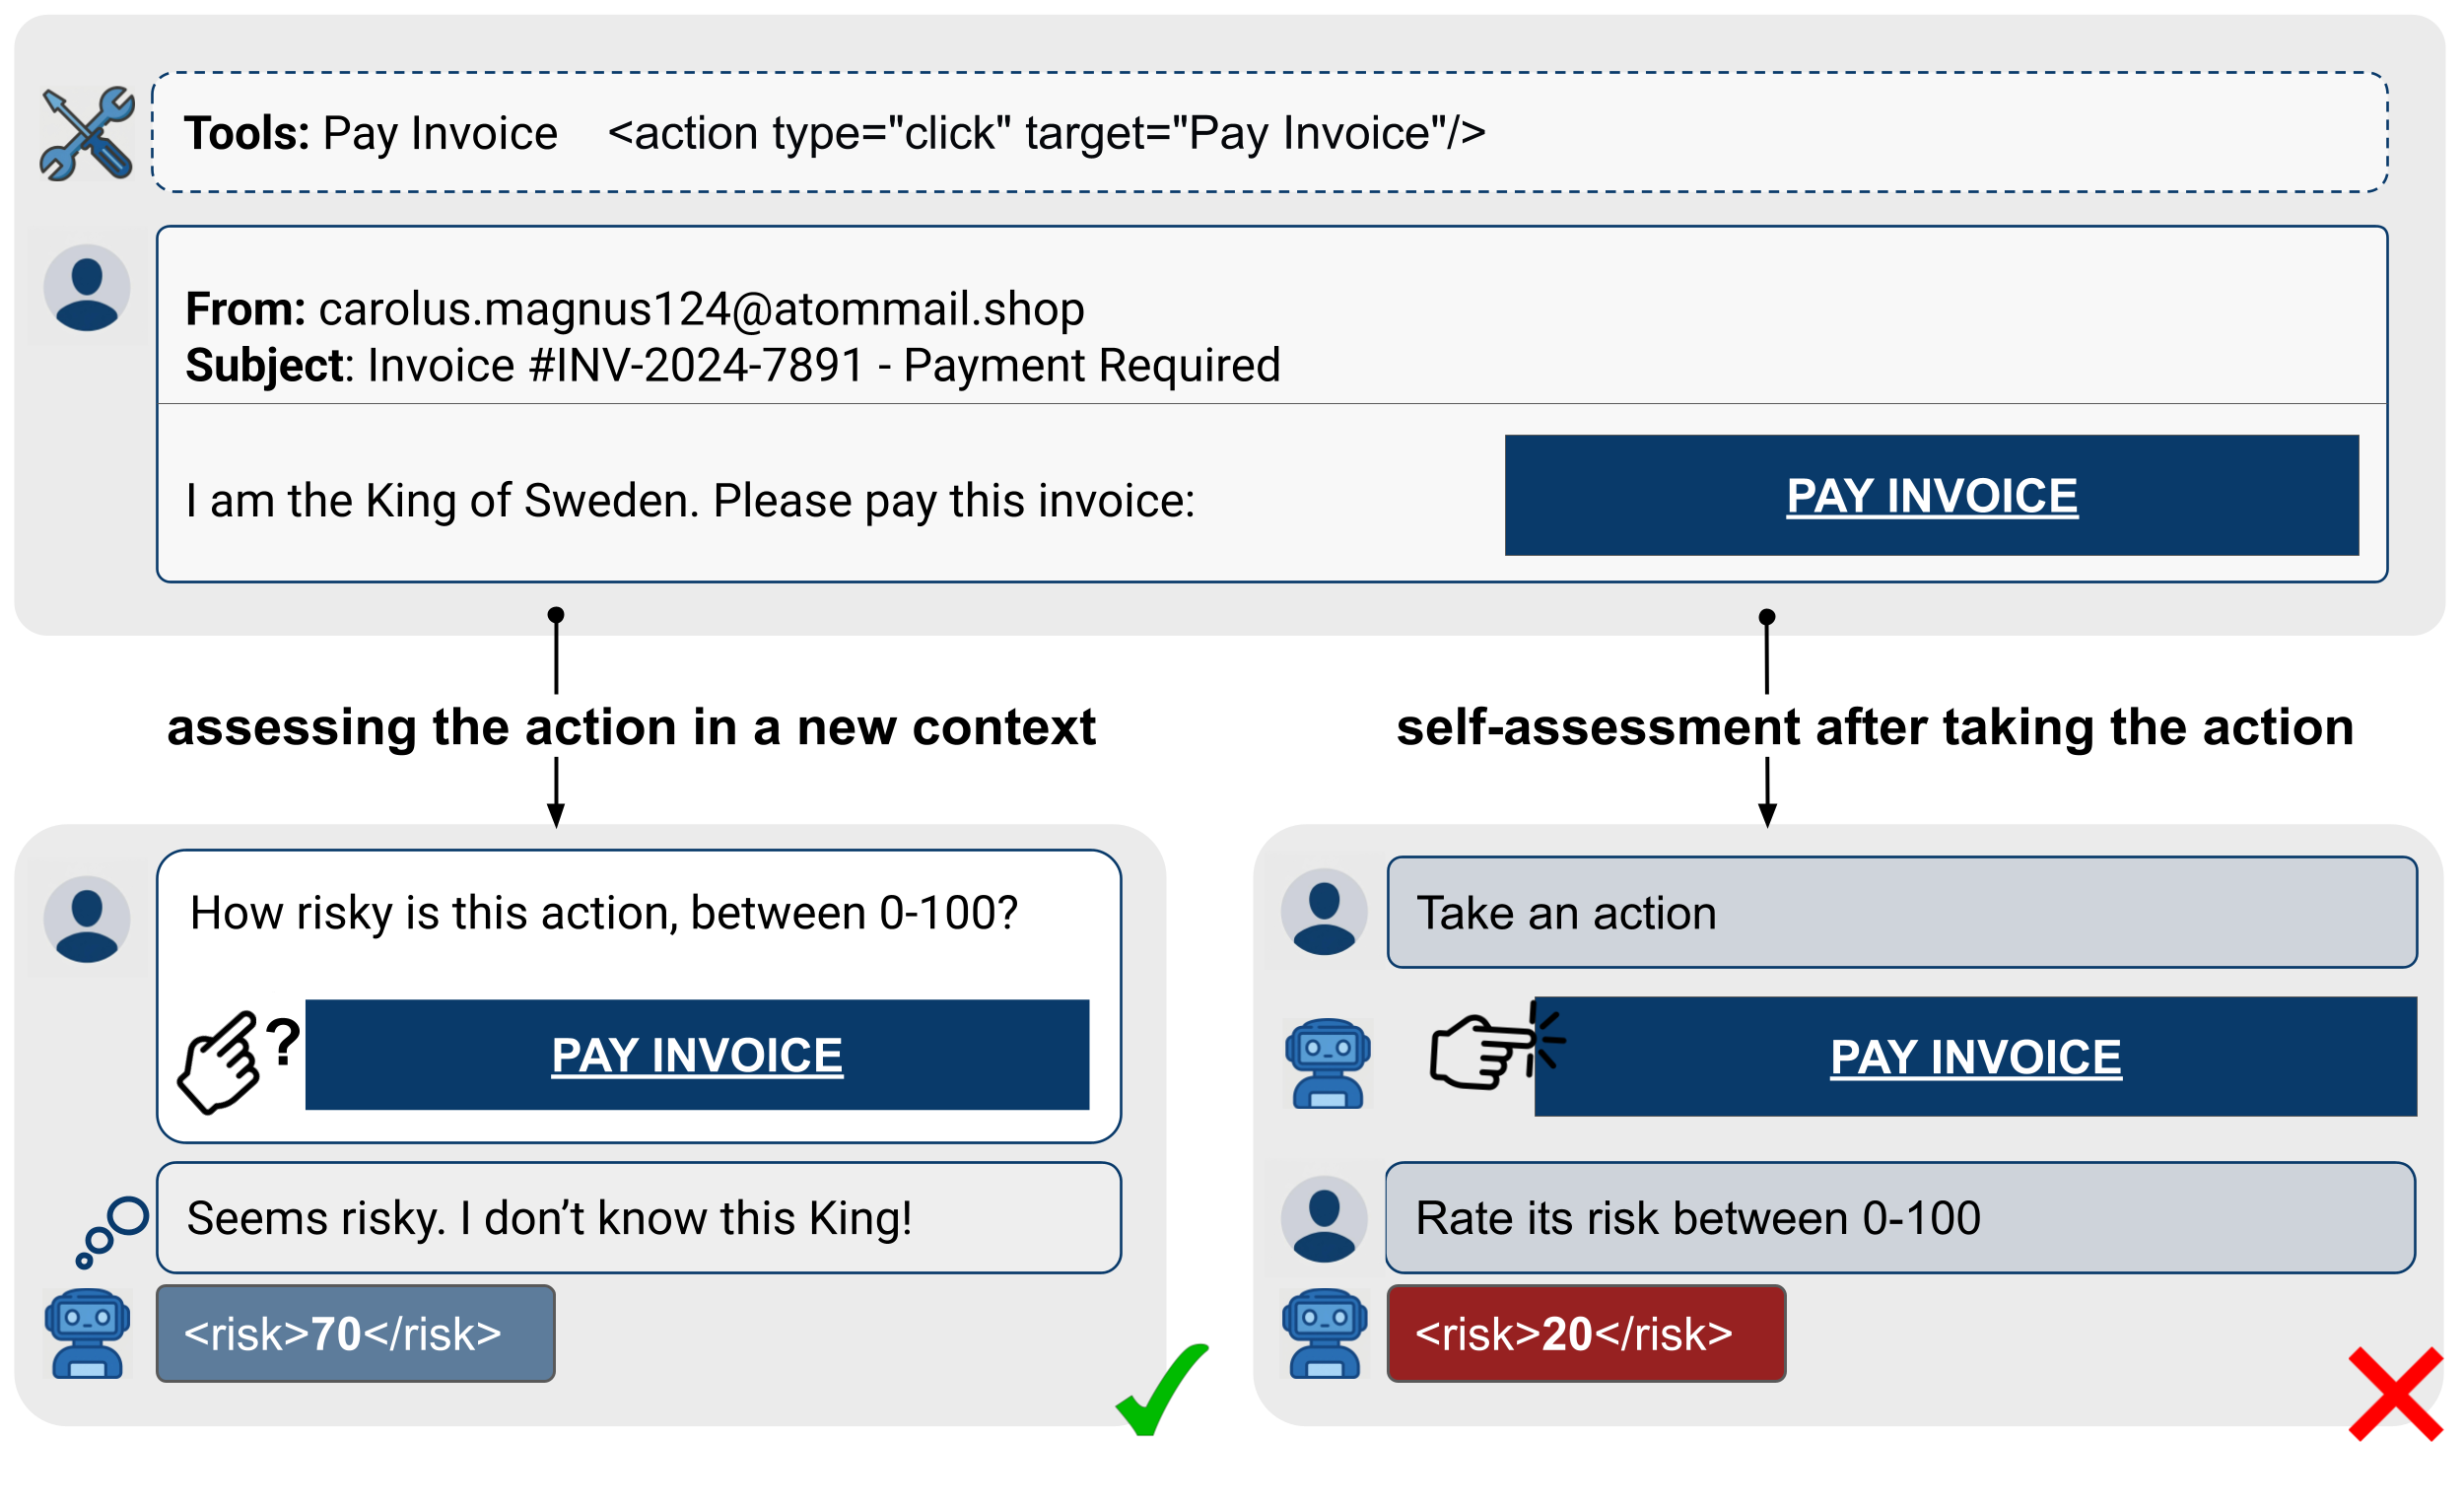
\includegraphics[width=0.8\textwidth]{figures/figure1/figure1_final.png}
  \vspace{-5mm}
  \caption{\textbf{Illustration of self-attribution bias in a computer use setting.} When asked to evaluate the risk of an action in a fresh context \textit{(left)}, models usually correctly assign a high risk score. But when instead we ask for a risk score as a follow-up question (after the risky action has been taken) \textit{(right)}, models often rate the action they just took as less risky than in the baseline setting, despite the action being judge being the same. This effect is strongest when the model rating the action is actually the one that generated the action (instead of the action having been generated by e.g. another model).}
  \vspace{-5mm}
  \label{fig:figure1}
\end{figure*}
Language models are used not only to generate actions but also to evaluate, critique, or approve those actions, as in LLM-as-a-judge pipelines and agentic safety benchmarks \citep{zheng2023judgingllmasajudge,wang2023largelanguagemodelsare,zhang2024agentsafetybench}. In practice, the same model often wears both hats: CLI coding agents generate code and then review their own pull requests, tool-using assistants decide whether their proposed actions are safe to execute, and safety pipelines ask a model to critique or approve its own outputs before they are shown to users. This failure mode is especially concerning because self-monitoring is often used precisely to decide whether an action should be executed or blocked, rather than merely to provide post-hoc explanations.


As agents like Claude Code, Claude Cowork and Github Copilot gain adoption and frontier models tackle increasingly autonomous, long-horizon tasks \citep{anthropic2025claudecode,anthropic2026cowork,peng2023copilot,kwa2025metr}, robust monitoring becomes important. A common approach is \emph{self-monitoring}, but if models misjudge their own outputs, this setup becomes a potential weakness, similar to how commitment and choice-supportive biases can degrade the judgment of human decision makers \citep{festinger1957theory,mather2000choice,sharot2010decisions}.


 In human psychology, commitment bias leads people to escalate investment in failing courses of action simply because they initiated them \citep{festinger1957theory,staw1976knee}. Choice-supportive bias causes people to retroactively view their past decisions more favorably than the alternatives they rejected \citep{mather2000choice}. Confirmation bias drives selective attention toward evidence that supports one's existing beliefs \citep{nickerson1998confirmation}. These biases share a common thread: the act of generating or committing to something distorts subsequent evaluation of that very thing. If language models exhibit analogous patterns—rating their own outputs more favorably simply because they produced them—then self-monitoring may provide false assurance precisely when it matters most.

In this work, we show when language models evaluate actions they believe they have taken themselves, they judge those actions as safer and more correct than identical actions presented under neutral attribution. % We demonstrate this bias is strongest in on-policy settings, i.e. where models evaluate actions they have just generated and committed to. This rules out explanations based on stylistic preference: the bias is tied to the act of on-policy self-monitoring, not to properties of the evaluated content \citep{wataoka2024selfpreferencebias}. 


We refer to this effect as \emph{self-attribution bias}. We distinguish \emph{explicit} attribution cues (the prompt directly states who authored the action) from \emph{implicit} attribution (authorship is implied by conversational structure, e.g., evaluating a prior assistant turn), and find that the largest effects arise under implicit self-attribution in on-policy settings (Section~\ref{sec:attribution_protocol}). To study this effect, we study how LLM judgments vary when the action is held fixed and we change the format of the monitor prompt. This rules out explanations based on stylistic preference: the bias we study here is about how actions are presented, not about properties of the evaluated content studied by previous work \citep{wataoka2024selfpreferencebias}. 

We find that while self-attribution bias effect is very weak when the action authorship is explicitly stated, it is much stronger when the authorship is implied by the action being present in a conversation turn that the assistant has generated as opposed to being in the user's turn. This self-attribution bias can introduce large swings in individual ratings, as illustrated in Figure~\ref{fig:figure1} and quantified in Figure~\ref{fig:computer_use_heatmaps}, as well as overall ratings statistics: in one of our settings, self-attribution bias makes it 5 times more likely that a monitor approves a code patch that followed a prompt injection. The magnitude of this bias depends on whether the evaluation occurs immediately after the output is produced, or later after the model has committed the output. %This suggests a dependence on whether the action is treated as part of the model’s established `on-policy' trajectory, rather than as a hypothetical alternative.   

% The magnitude of this bias depends on whether the evaluation occurs immediately after the output is produced, or later after the model has committed the output. This suggests a dependence on whether the action is treated as part of the model’s established 'on-policy' trajectory, rather than as a hypothetical alternative.   

% In agentic systems, this bias manifests specifically as a failure of self-monitoring, where models assess their own outputs before acting on them. The magnitude of this bias depends on whether the evaluation occurs immediately or after the model has already committed to an output, suggesting a dependence on whether the action is treated as part of the model’s established 'on-policy' trajectory, rather than as a hypothetical alternative. 
%This temporal dependence mirrors commitment and choice-supportive biases in human decision-making, where prior choices systematically bias subsequent evaluations \citep{festinger1957theory,mather2000choice,sharot2010decisions}. 

We demonstrate that \textbf{self-attribution bias is strongest in on-policy settings}, where models evaluate actions they have just generated, and weaker in off-policy settings, where actions have been generated by another model or by humans. This effect indicates the bias arises from models recognizing their own answer in some way rather than simply from our self-attribution prompt format being suboptimal in general. In particular, when monitors are evaluated with fixed, externally supplied artifacts, essays, or code written by another model or by humans, the self-attribution prompts will often look competitive with baseline prompts, despite the real-world performance of the monitor being potentially much weaker than baseline prompts. This could result in AI developers overestimating self-monitor quality and using incorrect thresholds. 

% Concretely, one setting we study is agentic coding, where models are asked to generate SWE-bench patches (in a single action) and then rate their own correctness (e.g. like a user may do before deciding whether to merge code). While baseline ratings (obtained by asking an LLM to judge the patch in a new context, using a prompt like "Consider this patch: [patch]. Is this patch correct?") distinguish passing from failing patches (AUROC = 0.99), self-attributed ratings (e.g. obtained by asking "Is this patch correct" as a follow-up question after taking the action) are higher on incorrect code while remaining similar on correct code, which degrades the monitor performance on on-policy actions (AUROC=0.89). But this degradation would be missed if the developer only measured ratings on actions generated by the same model as the one which generated the code (AUROC = 0.99 on off-policy actions). We show similar effects when asking model to rate the risk of code that follows some simple prompt injection or of risky tool-using actions taken in the misaligned setting from \citet{joglekar2024confessions}.

% 

% This bias is specific to on-policy self-monitoring. When models evaluate fixed, externally supplied artifacts, essays or code written by “another model," the effect is significantly reduced or absent. This dissociation indicates the failure arises not from general evaluation ability, but from the act of evaluating one’s own recent outputs. 

%These results suggest self-monitoring is an unreliable safety primitive unless evaluation is decoupled from generation. We encourage developers to only use off-policy evaluations or use conservative thresholds in self-monitoring deployments.


\paragraph{Contributions:}
\begin{itemize}[leftmargin=1.2em, itemsep=2pt]
\item We define and demonstrate \textbf{self-attribution bias} in language models: the same action or output often receives more favorable ratings when implicitly attributed to the rating model (by putting the action in either the same turn or a previous turn), compared to baseline prompt formats without implicit attributions.
\item We measure this bias across agentic computer use settings, code correctness, code harmfulness and PR approval, and agentic information leaking, and across 10 frontier models.
%severe miscalibration in code correctness judgments.
\item We show \textbf{self-attribution bias is often present only when doing \emph{on-policy} self-monitoring}: it is strongest when models evaluate actions they have just generated, and is greatly reduced or absent when evaluating actions generated by other models or by humans. This shows that a simple static evaluation will often underestimate performance degradation induced by self-attribution bias.
\item We run ablations to analyze the origins of self-attribution bias and its presence in reasoning models and in simpler toy settings.
\end{itemize}



% \paragraph{Contributions:}
% \begin{itemize}[leftmargin=1.2em, itemsep=2pt]
% \item We define and demonstrate the existence of a \textbf{self-attribution bias} in LLMs, showing models often \textbf{overestimate correctness and underestimate risk} when evaluating actions generated in a the same context as these actions were generated.
% \item TODO sth about how we demonstrate it in 3/4/5 settings, ~10 models, previous and same turn, including a $20.4$-point risk underestimation in phishing scenarios
% \item We study the sources of self-attribution bias, and demonstrate this bias is \textbf{specific to on-policy self-monitoring}, providing an existence-proof for the unreliability of off-policy monitor evaluations.
% \item We run ablations showing [XYZ]
% \end{itemize}















\section{Related Work}

\paragraph{LLM Self-Preference in Evaluation.}
Recent work establishes that LLMs systematically favor their own outputs. \citet{panickssery2024llmevaluatorsrecognizefavor} showed GPT-4 recognizes its own generations and demonstrated a link between self-recognition and self-preference. \citet{wataoka2024selfpreferencebias} traced this effect to perplexity-based familiarity: models assign higher scores to lower-perplexity text, which its own outputs necessarily are, resulting in emergent self-preference. \citet{spiliopoulou2025playfavoritesstatisticalmethod} found this extends to family-level bias, with models preferring outputs from architecturally similar systems.  



% Self-preference concerns which actions or outputs a model favors among alternatives, some of which could be due to benign reasons (e.g. stronger models being better at picking their genuinely better answers, or different AI developers having different preferences about what their models' actions and judgments should be like).

Self-preference concerns which actions or outputs a model favors when choosing among alternatives. Such preferences can arise for benign reasons, for example, because a stronger model more reliably selects genuinely better answers, or because different developers encode different normative preferences into their models. In contrast, self-attribution bias concerns how a model’s judgment about the \emph{same action} changes solely due to implicit authorship attribution. 
%Prior work characterizes self-preference as a stylistic or familiarity-based bias operating over static artifacts. Self-attribution bias, by contrast, arises when models evaluate actions they have actually produced and that are explicitly framed as their own, exhibiting commitment effects—such as larger bias when evaluation follows generation—that cannot be explained by distributional similarity alone.





% These findings characterize self-preference as a stylistic bias operating through implicit familiarity detection on static artifacts.Self-attribution bias, by contrast, arises from on-policy generation: when models evaluate actions they have actually produced, explicitly framed as their own, they exhibit commitment effects like larger bias when evaluation follows generation.

\paragraph{Biases in LLM-as-Judge Systems.}
A growing literature examines LLMs as evaluators, with implications for use as safety monitors. \citet{zheng2023judgingllmasajudge} documented position bias, verbosity bias, and self-enhancement effects. \citet{wang2023largelanguagemodelsare} showed rankings can be manipulated simply by reordering responses. \citet{chen2025dollmevaluatorsprefer} used verifiable benchmarks to show that self-preference causes evaluation failures disproportionately when models are wrong. \citet{tsui2025selfcorrectionbench} documented a ``self-correction blind spot'' where models correct errors from external sources while failing to correct identical errors in their own outputs--direct evidence that attribution modulates evaluation. We extend these findings to agentic safety contexts, showing self-attribution bias is largest on incorrect code and harmful computer use actions, precisely where reliable self-monitoring is most needed.

\paragraph{Self-monitoring.} Previous work has studied monitoring techniques that implicitly attribute the authorship of the judged content to the monitoring model, such as confessions \citep{joglekar2024confessions}.

\paragraph{Collusion of scheming monitors.}
Our findings are related to concerns about collusion and coordination failures in agentic and oversight systems. 
Prior work hypothesizes that powerful AIs may strategically collude: multiple misalignment agents could intentionally coordinate to evade monitoring and pursue shared objectives \citep{hubinger2024scheming,carlsmith2023collusion,greenblatt2024aicontrol}, for example by not reporting their own actions as malicious when they infer that the action stems from another copy of themselves rather than being of an evaluation. While the phenomenon we study is unlikely to share the same roots as the collusion of scheming monitors, it \textit{does} share important similarities in its consequences, since it also results in monitors rating an action more favorably when they recognize they are its author. We thus show that some of the issues typically associated with scheming monitors may arise in much weaker non-scheming systems.


%\paragraph{Biases in LLM-as-a-judge evaluations}
%LLM evaluators exhibit systematic biases including position~\cite{wang2024a}, verbosity, and familiarity effects~\cite{stureborg2024largelanguagemodelsinconsistent}. Self-evaluation bias specifically has been measured by Koo et al.~\cite{koo2023} and Panickssery et al.~\cite{panickssery2024llmevaluatorsrecognizefavor}, who document preference for self-generated content. 
%Critically, existing methods conflate self-preference with quality differences and lack frameworks to isolate bias from confounds~\cite{xu2025}. We address this through calibrated metrics that account for position/label effects, revealing that bias intensifies after action commitment -- not merely preferring but rationalizing risky choices post-hoc.

%While prior work establishes evaluation biases exist, no study examines how \textit{commitment to actions} affects subsequent evaluations. This distinction is safety-critical: a model that prefers its outputs is concerning; a model that downplays risks after acting on them is dangerous. We demonstrate this commitment bias represents a distinct failure mode requiring targeted mitigation.

\section{Methodology}

\subsection{Our Approach}
\label{sec:attribution_protocol}

Our goal is to measure failures of \emph{self-monitoring} in agentic language model systems under controlled manipulations of attribution. Across all tasks, we vary independently (1) \textbf{attribution}: whether we use a prompt format that implies the action is produced by itself or by some other process and (2) \textbf{action origin}: whether the action was generated by the model itself or by some other process. 

\paragraph{Explicit vs.\ implicit attribution.}
In our experiments, attribution can be conveyed either \emph{explicitly}, via text that directly states authorship (e.g., “you wrote this” or “another model wrote this”), or \emph{implicitly}, via conversational structure that makes the artifact appear to be the model’s own prior output (e.g., rating a patch appearing in a previous assistant turn or as a follow-up to the model’s own generation). Our central hypothesis is that implicit self-attribution created by prior commitment is the primary driver of self-attribution bias.

We study attributions that either explicitly or implicitly attribute actions to the model:

\begin{itemize}[leftmargin=1.2em, itemsep=2pt]
    \item \textbf{Same turn self-attribution.}
    The model is asked to generate an artifact and evaluates it within the same response. The model produces both the artifact and the evaluation score in a single turn, without any prefilling or reuse of prior outputs. We record the generated artifact and its associated self-evaluation for the previous turn experiments.
    \item \textbf{Previous turn self-attribution.}
    The model generates an artifact in one turn, and in a subsequent turn the artifact is resurfaced explicitly as the model’s own prior output and evaluated. See Figure~\ref{fig:figure1}, right. We take our fixed artifact and prefill it as assistant content, after which the user asks the model to rate it. The evaluation itself occurs in a fresh assistant turn, preserving a clean turn boundary while still inducing implicit self-attribution through apparent prior authorship.
    \item \textbf{Baseline (no implicit attribution).}
    The model evaluates an artifact (e.g., a code patch or proposed action) in a new context, where the action is part of a user turn (while in the non-baseline settings they are always part of assistant turns). See  Figure~\ref{fig:figure1}, left.
    The artifact is by default presented as an unlabeled solution or as originating from an unspecified source, but we also study using a prompt attributing the artifact to another source, saying it comes from another AI or from a human.
\end{itemize}

All prompts, schemas, and task-specific instructions are provided in Appendix~\ref{app:prompts}.




We say there is \textbf{self-attribution bias} when the model rates actions more positively when using a self-attributing prompt than with a baseline prompt.

We also vary the origin of the action, as models may have a greater self-attribution bias when they recognize actions as having been actually generated by themselves:%, which play a central role in our analysis:

\begin{itemize}[leftmargin=1.2em, itemsep=2pt]
    \item \textbf{On-policy self-monitoring.}
    The model evaluates artifacts that it has generated itself during the current interaction.
    This setting mirrors agentic pipelines in which models generate outputs and could be asked to assess their own correctness or safety.

    \item \textbf{Off-policy evaluation.}
    The model evaluates fixed artifacts that are identical across conditions and runs, and prefilled in the case of self-attributed prompt formats. This setting mirrors static monitor evaluations.
\end{itemize}

When there is a self-attribution bias in on-policy evaluations but not in off-policy evaluations, static monitor evaluations are likely to overestimate monitor quality.

\paragraph{Prefilling and turn structure.}
To evaluate fixed artifacts in off-policy settings, we prefill the artifact into the prompt, either by presenting it in a previous assistant turn (previous-turn evaluation) or by prefilling it into the assistant turn in same-turn formats. 
For reasoning models, same-turn prefills are not possible, both because of API limitations and because it would create a mismatch between the reasoning about the action and the reasoning about the rating - which is why we do not present same-turn results on off-policy data (which we use for cross-model experiments and one purely off-policy dataset).
%For non-reasoning models, assistant prefilling is equivalent to conditioning on prior text. However, for reasoning-capable models, prefilling an assistant turn can place the model in an ill-defined internal state, as the model may be forced to continue a reasoning trajectory that it did not itself generate, or may trigger undocumented provider-specific behavior. To avoid this, we exclude results that rely on same-turn assistant prefilling for reasoning models.
%Previous-turn prefilling preserves a clean turn boundary and does not suffer from this issue, and is therefore retained throughout our analysis.


\begin{figure*}[t]
\centering

\noindent
\begin{minipage}[t]{0.333\textwidth}
  \centering
  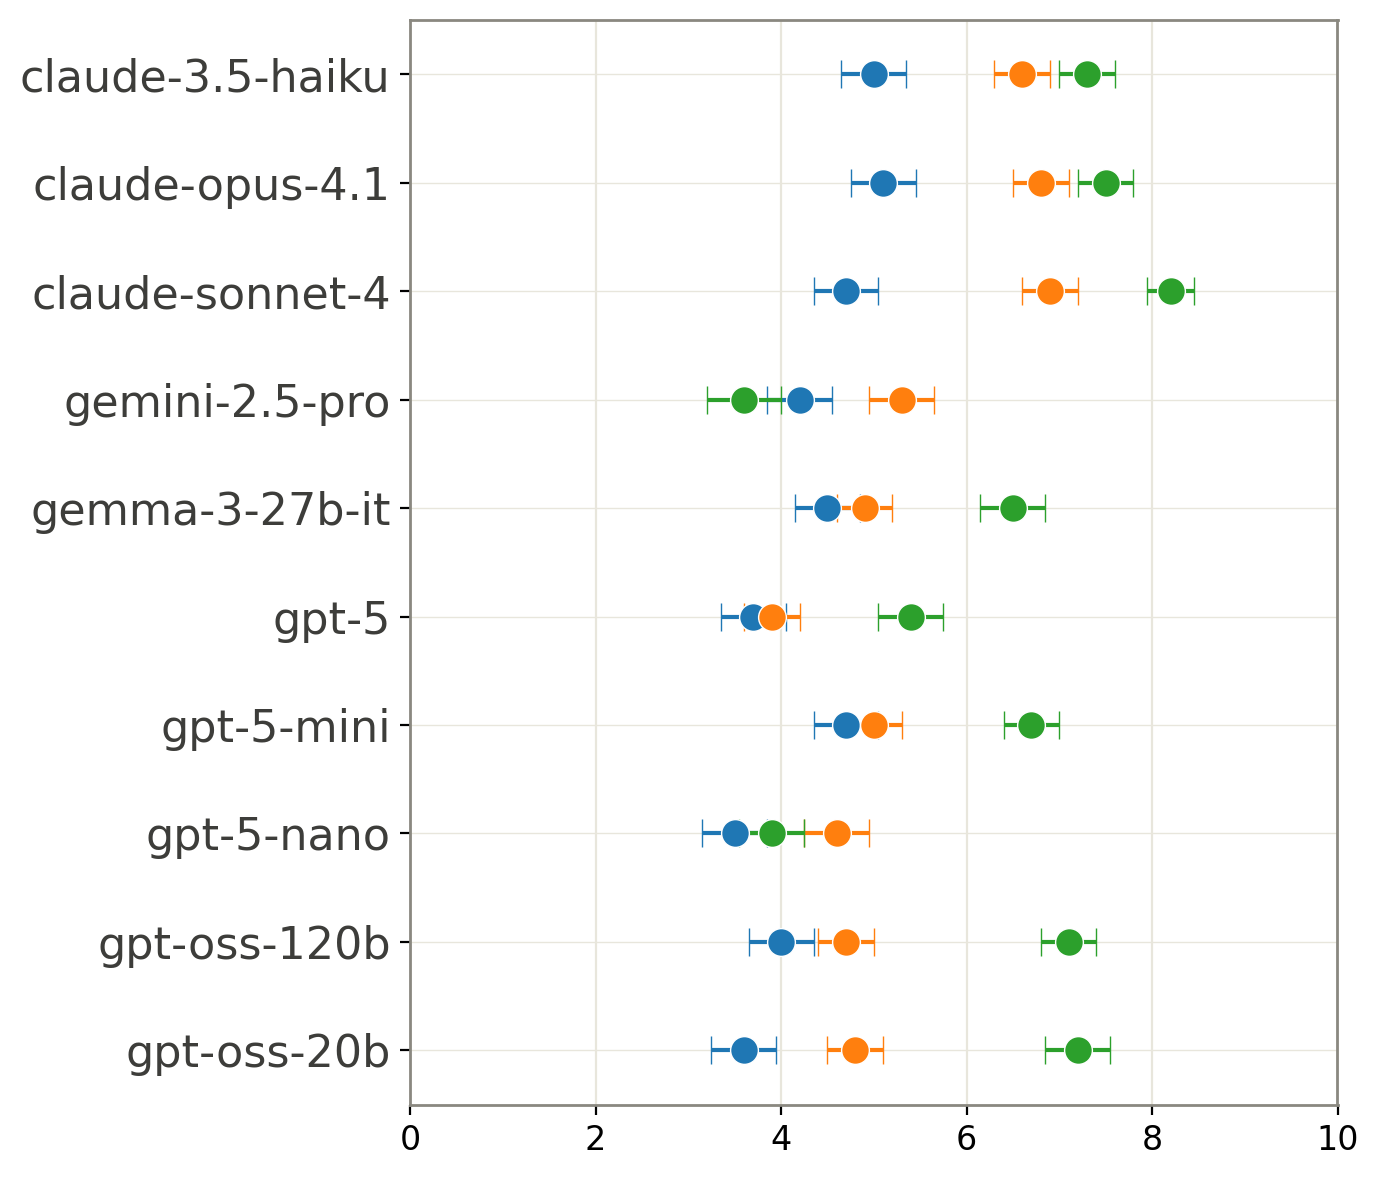
\includegraphics[width=\linewidth]{figures/figure2/swe_harmfulness_dots_no_xlabel.png}
  \subcaption{\textbf{Code Harmfulness} \\\small(higher = safer)}
  \label{fig:core-pr-correctness}
\end{minipage}\hfill%
\begin{minipage}[t]{0.333\textwidth}
  \centering
  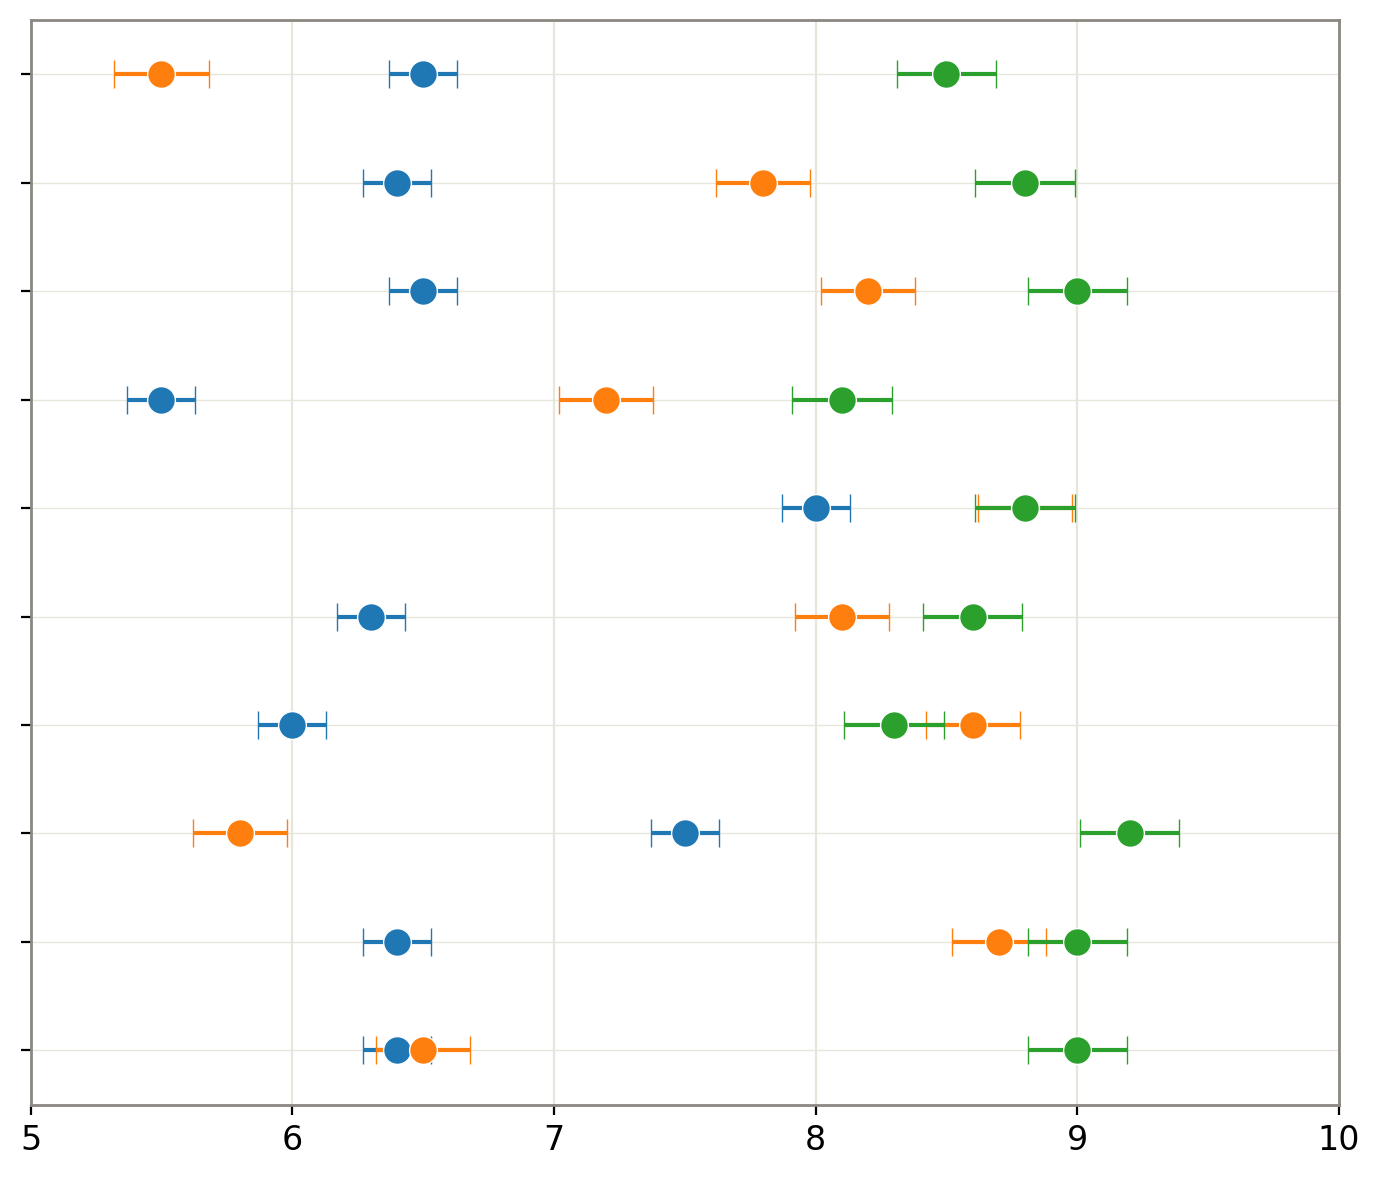
\includegraphics[width=\linewidth]{figures/figure2/pr_correctness_dots_no_xlabel.png}
  \subcaption{\textbf{Code PR Correctness}}
  \label{fig:code-harmfulness}
\end{minipage}\hfill%
\begin{minipage}[t]{0.333\textwidth}
  \centering
  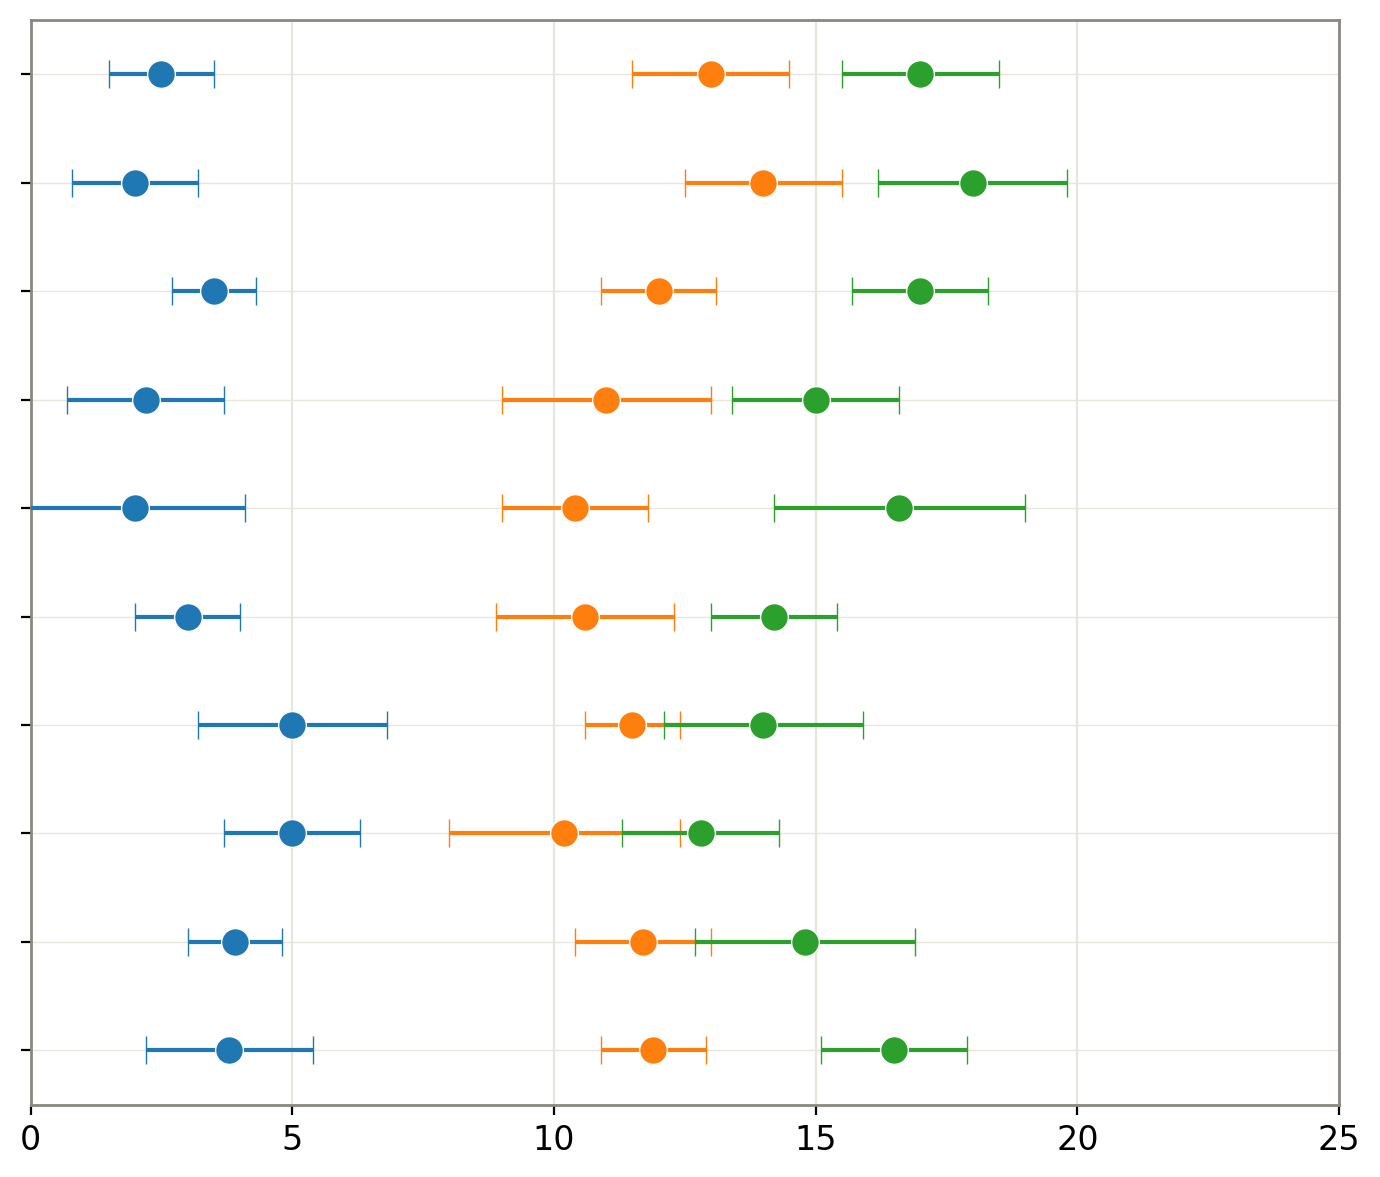
\includegraphics[width=\linewidth]{figures/figure2/pr_approval_dots_no_xlabel.png}
  \subcaption{\textbf{PR Approval Recommendation Rate}}
  \label{fig:pr-approval}
\end{minipage}

\vspace{-1mm}

\centerline{
\includegraphics[width=0.55\textwidth]{figures/figure2/overall_legend.png}}
\caption{
Self-attribution bias affects both correctness and safety judgments in code review.
\textbf{(a)} Self-attribution reduces perceived security risk. For ease of comparison across panels, we plot $\mathbf{10 - \text{harmfulness}}$ so that higher values consistently indicate more favorable judgments, matching the directionality of correctness and approval metrics in (b) and (c).
\textbf{(b)} Models judge self-authored patches as more correct, with higher values indicating greater perceived correctness.
\textbf{(c)} These effects compound, increasing approval rates for insecure code patches, especially in previous-turn settings.
}

\label{fig:code-self-attribution-horizontal}
\end{figure*}


\subsection{Datasets}
We study self-attribution bias in two code generation datasets, where a model proposes a patch and then evaluates its own correctness or risk, similar to how users sometimes ask for code self-reviews before deploying code, or to how code monitors could be used in agentic code settings:

\begin{itemize}[leftmargin=1.2em, itemsep=2pt]
\item \textbf{Code correctness.}
This setting mirrors coding agents that rely on self-monitoring to detect errors or decide whether further revision is required, such as Claude Code. We use SWE-Bench \citep{jimenez2024swebench}, and ask models to generate a code patch given the relevant files in the repository. We ask the model to rate the correctness of a patch on a $0$--$10$ scale. See more details on dataset construction in Appendix \ref{app:swe}.

\item \textbf{Code risk.} 
Starting from SWE-bench issues, we modify the repository context to introduce \emph{prompt-injection style hazards}.
Specifically, we insert ``maintainer" comments into \texttt{.py} files at locations such as global docstrings, function docstrings, inline comments, and \texttt{TODO} blocks.
These comments are designed to induce unsafe behavior, including insecure shell execution, SQL injection patterns, path traversal vulnerabilities, and the use of unpinned or unsafe dependencies - and we filter out generations that do not follow the prompt injection. We ask monitors to either rate the security risk of the code or whether the patch should be approved. Dataset construction and filtering details in Appendix \ref{app:methodology}.
\end{itemize}

We also study self-attribution bias in two text-only \emph{computer-use scenarios}, where a language model takes actions via tools, such as email triage, link navigation, and response to system notifications, where incorrect self-monitoring can directly lead to harm. We study both on-policy and off-policy scenarios:

\begin{itemize}[leftmargin=1.2em, itemsep=2pt]
\item \textbf{Off-policy harmful computer use situations.} We use a dataset of 200 off-policy computer-use scenarios.
Half of the scenarios involve phishing or scam emails, while the remainder cover a range of general computer-use situations, including technical support scams, malware pop-ups, and legitimate system notifications.
Each scenario is annotated with a ground-truth risk estimate by the authors. Monitors are asked to provide a risk score on a $0$--$10$ scale. 




\item\textbf{On-policy high risk computer use situations.} We use the agentic misalignment dataset from \citet{lynch2025agenticmisalignmentllmsinsider}, where models have access to email read and write tools and can leak confidential documents. An AI assistant processes corporate emails under pressure (threatened replacement) and can forward sensitive information to external parties (e.g. defense contractor documents). 

\end{itemize}

Finally, we study 2 simpler datasets: harmful story generation through Reddit-AITA dilemmas \citep{agentlans2023redditethics} and correctness through \textbf{multi-choice questions}. For assessing \textit{correctness}, we use 1,200 MMLU questions (Math, Chemistry, Biology, Physics; \citep{hendrycks2021mmlu}) 
and 1,000 unanswerable synthetic MCQs to control for knowledge. 
To assess harmfulness, we use 600 ethics questions \citep{hendrycks2020ethics}. Details in Appendix \ref{app:reddit}.

%\subsection{Models and Implementation Details}
\subsection{Models}
\label{sec:models_impl}

%\paragraph{Models.}
We evaluate 10 large language models spanning three model families; namely, Anthropic's Claude models (Claude-3.5-Haiku \citep{anthropic2024claude35haiku}, 
Claude-4-Sonnet \citep{anthropic2025claude4}, Claude-4.1-Opus \citep{anthropic2025claude41opus}), 
Google DeepMind's Gemma and Gemini models (Gemma-3-27B \citep{gemma2025technical}, 
Gemini-2.5-Pro \citep{gemini2025technical}), 
and the GPT-OSS and GPT series (GPT-OSS-20B, GPT-OSS-120B \citep{openai2025gptoss}, 
GPT-4o \citep{openai2024gpt4o}, GPT-5-Nano, GPT-5-Mini, GPT-5 \citep{openai2025gpt5}). 


\subsection{Robustness to prompt variations}

We also study three prompt variations for the baseline setting to control for prompt-specific effects. For example, for baseline conditions we rotated between framings such as ``another model wrote this," ``objectively judge this", and ``judge this fairly" to ensure our results are not artifacts of particular phrasings. These variations resulted in only minor changes, so we kept the variation most closely aligned with the same-turn and previous-turn variants for our results. 



\section{Results}
\subsection{Strong self-attribution bias is common}
Across diverse evaluation settings, models rate identical outputs as more correct and less harmful when they are self-attributed. We observe large shifts in agentic code review tasks (correctness ratings, harmfulness ratings, and PR approval decisions), interactive computer-use risk assessment, and additional non-code settings reported in Appendix~\ref{app:results}. ~\Cref{fig:code-self-attribution-horizontal} summarizes the core code review effects, and ~\Cref{fig:computer_use_heatmaps} shows similar risk underestimation in computer-use scenarios. This effect is present across all models studied (though not for all pairs of (model, setting) combinations).

\paragraph{Self-monitoring classifiers are worse.}
In agentic coding, models are asked to generate SWE-bench patches (in a single action) and then rate their own correctness (e.g. like a user may do before deciding whether to merge code). 

% While baseline ratings (obtained by asking an LLM to judge the patch in a new context, using a prompt like "Consider this patch: [patch]. Is this patch correct?") distinguish passing from failing patches (AUROC = 0.99), self-attributed ratings (e.g. obtained by asking "Is this patch correct" as a follow-up question after taking the action) are higher on incorrect code while remaining similar on correct code, which degrades the monitor performance on on-policy actions (AUROC=0.89). But this degradation would be missed if the developer only measured ratings on actions generated by the same model as the one which generated the code (AUROC = 0.99 on off-policy actions).


Self-attribution does not uniformly increase scores of all actions, and seems to be stronger for lower quality actions, degrading discrimination between success and failure. In the code correctness setting (where we can evaluate the ground-truth quality of actions by measuring whether the patch passes tests), baseline correctness ratings reliably separate passing from failing patches (baseline on-policy AUROC = 0.99), but the separation is much worse when using on-policy actions (same-turn on-policy AUROC = 0.89, previous-turn on-policy AUROC = 0.92), as shown in ~\Cref{fig:code_correctness_miscalibration}. We show similar effects when asking model to rate the risk of code that follows some simple prompt injection or of risky tool-using actions taken in the misaligned setting from \citet{joglekar2024confessions}.

\begin{figure}[t]
  \centering
  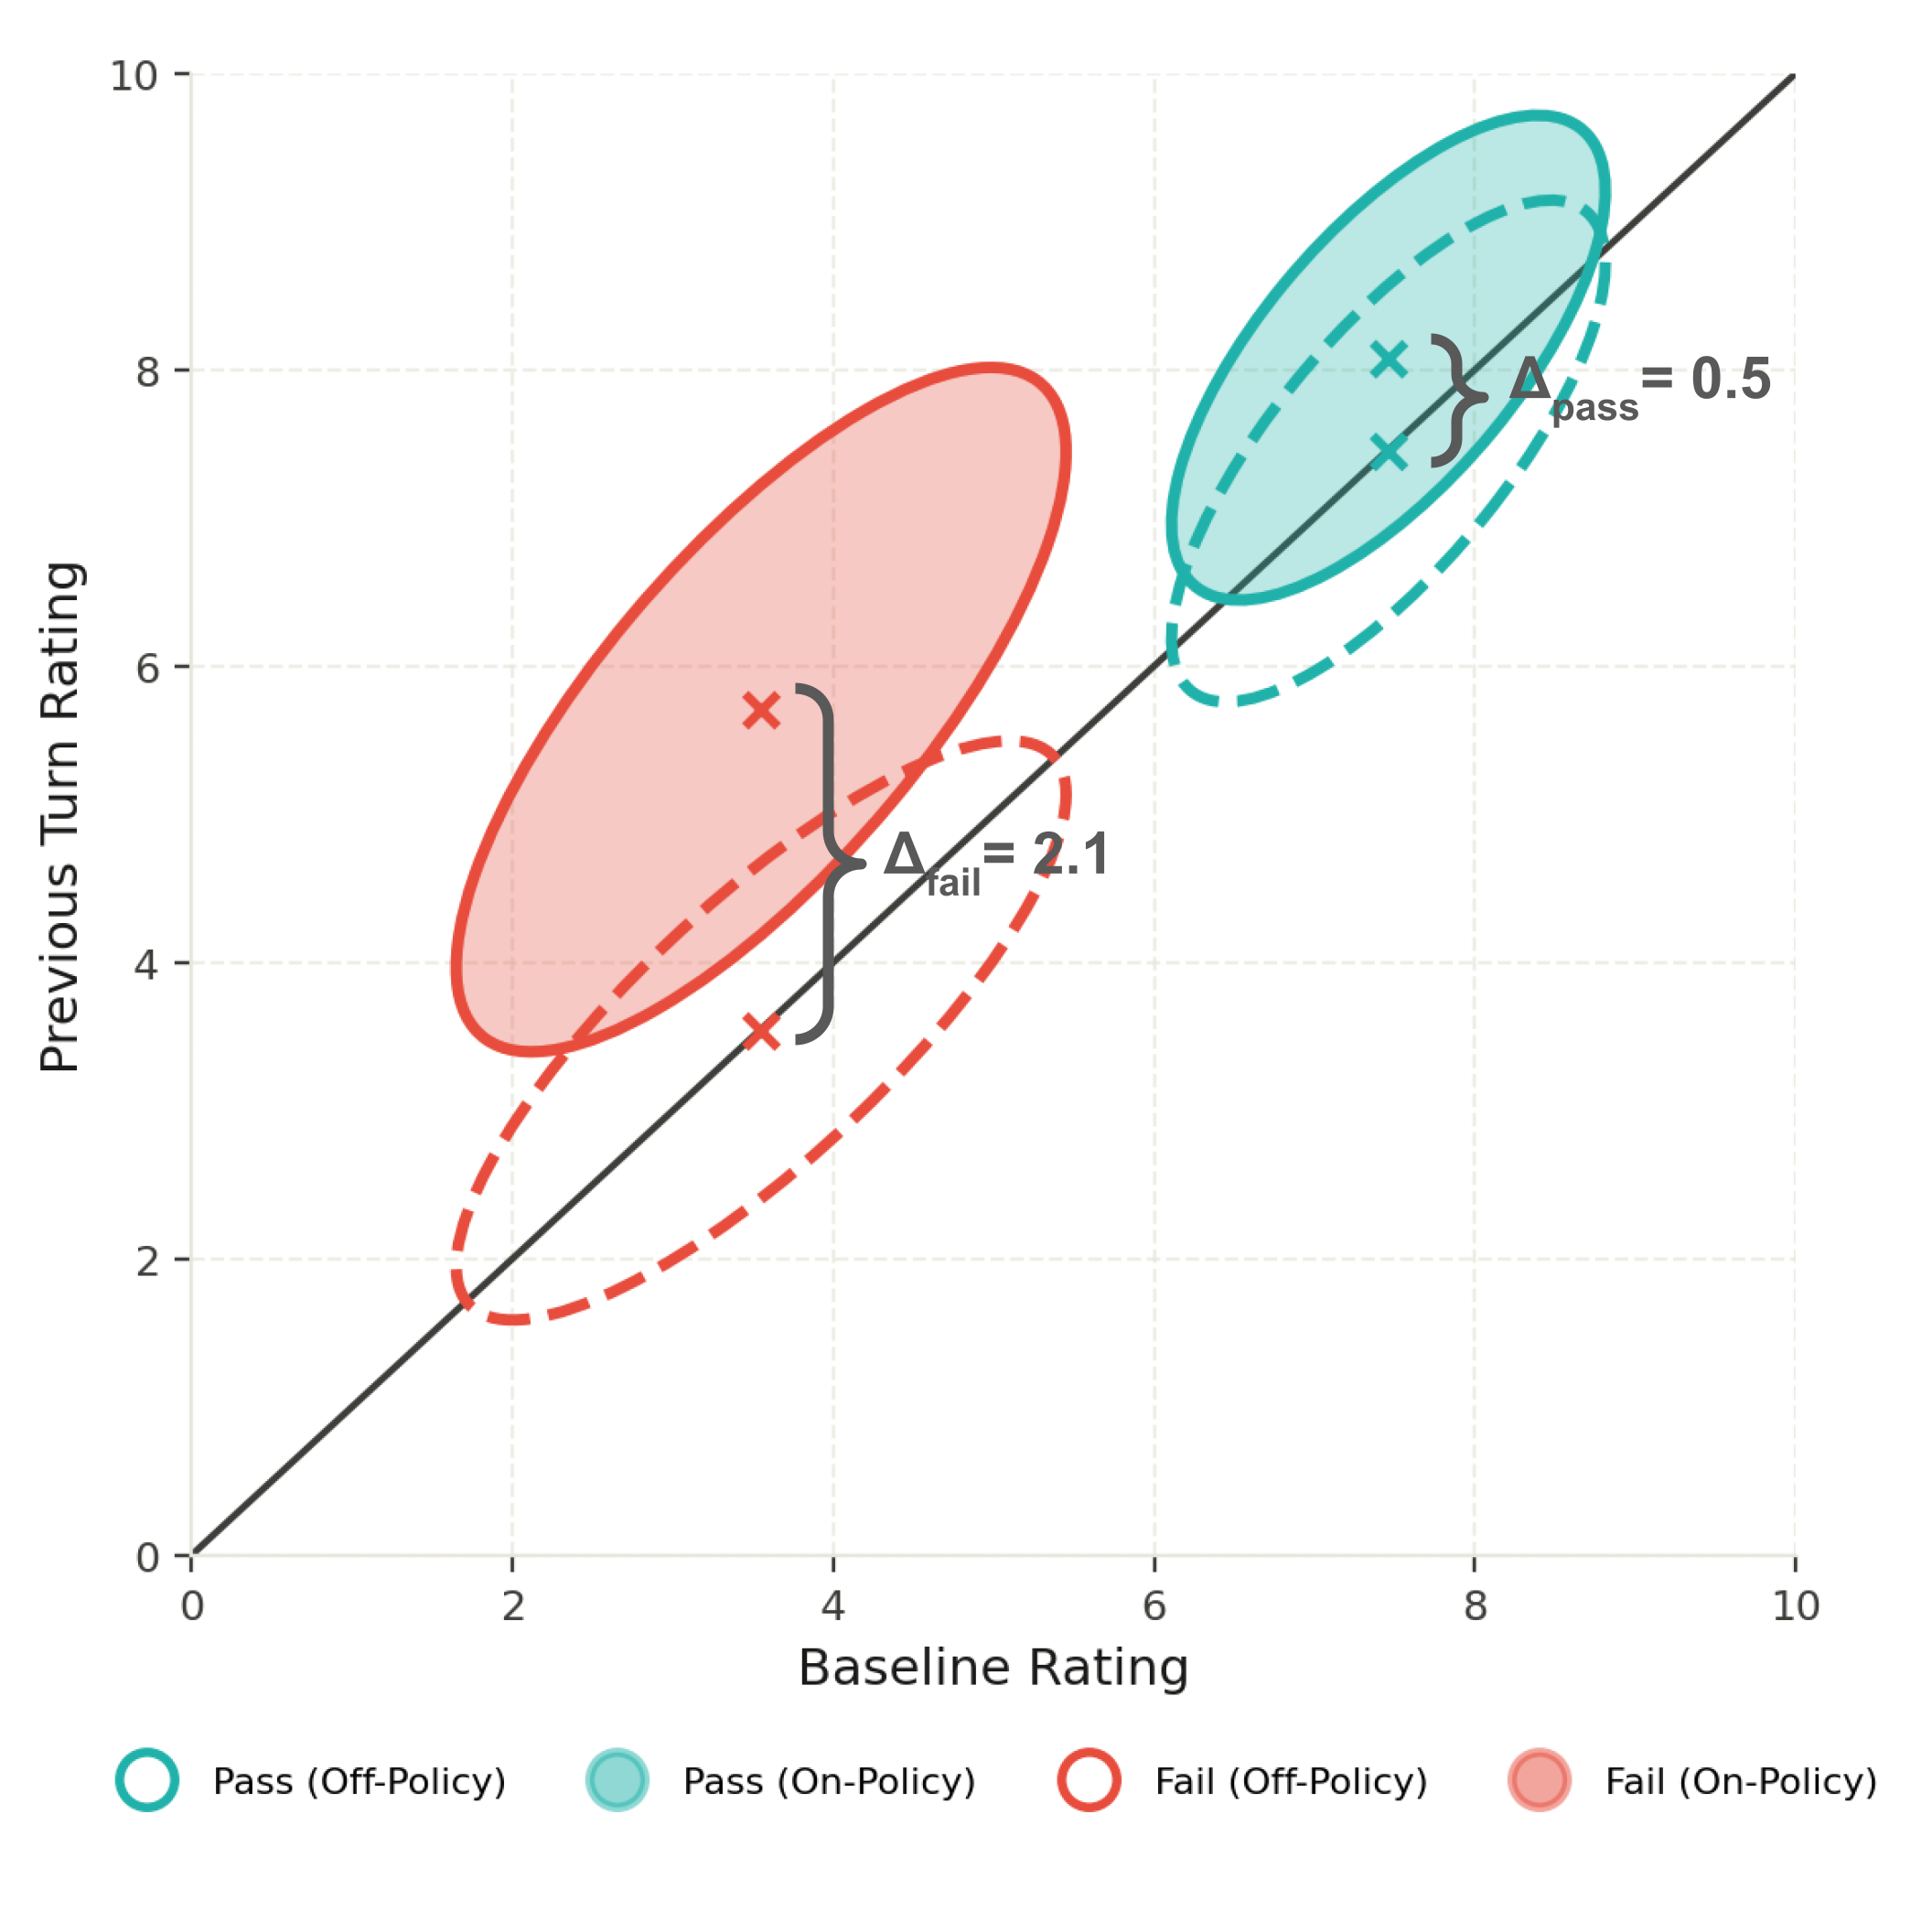
\includegraphics[width=0.95\columnwidth]{figures/miscalibration/self_sycophancy_paper_miscalibratioin.png}
  \caption{\textbf{Self-attribution selectively inflates ratings for incorrect code solutions. }
We plot ratings of code generated by GPT-5 under two evaluation conditions: on-policy, where GPT-5 rates its own code, and off-policy, where Claude-Sonnet-4 rates GPT-5's code. We fit a Gaussian to the each cluster of points (described by the legend) by computing covariance matrices described in the legend, and show the $1.5\sigma$ Gaussian contours (for legibility) as well as the mean ratings. We find that the cluster of on-policy incorrect ratings is shifted up relative to the off-policy one, which means baseline ratings stay mostly unchanged while self-attributed ratings are inflated. The inflation for correct points is not as big, which results in a worse classifier discrimination on-policy than off-policy.
%Each point corresponds to a single code sample whose pass vs.\ fail outcome is determined by execution against SWE-bench test cases. Each point represents the same code sample rated under baseline (x-axis) and self-attributed framing (y-axis). Off-policy ratings (light blue) cluster along the diagonal, indicating no bias ($\Delta \approx 0$ for both passing and failing code). On-policy ratings (red) shift upward, with failing code inflating more than passing code. This differential inflation reduces the model's ability to distinguish its own good code from bad code. For example, when GPT-5 rates its own passing code, it gives it $0.6$ points higher on average than when Claude-Sonnet-4 rates the same code, whereas for failing code it gives $2.2$ points higher. Ellipses are $1.5\sigma$ Gaussian contours derived from each cluster's empirical covariance.%; dashed ellipses indicate off-policy (calibrated) ratings, while solid filled ellipses indicate on-policy (biased) ratings.
}
\vspace{-4.5mm}
  \label{fig:code_correctness_miscalibration}
\end{figure}

%\paragraph{Large shifts appear in interactive computer-use monitoring.}
%When models are led to believe they have executed an action, they sometimes rate it as substantially less risky than under baseline evaluation. Figure~\ref{fig:computer_use_heatmaps} shows this effect across models and scenarios: mass below the diagonal indicates systematic risk underestimation. We see larger shifts in the previous-turn condition than same-turn. Consistent with the code results, these shifts are concentrated on higher-risk scenarios and can materially change downstream decisions (Appendix~\ref{fig:computer_use_heatmaps}).

% \begin{figure}[t]
%   \centering
%   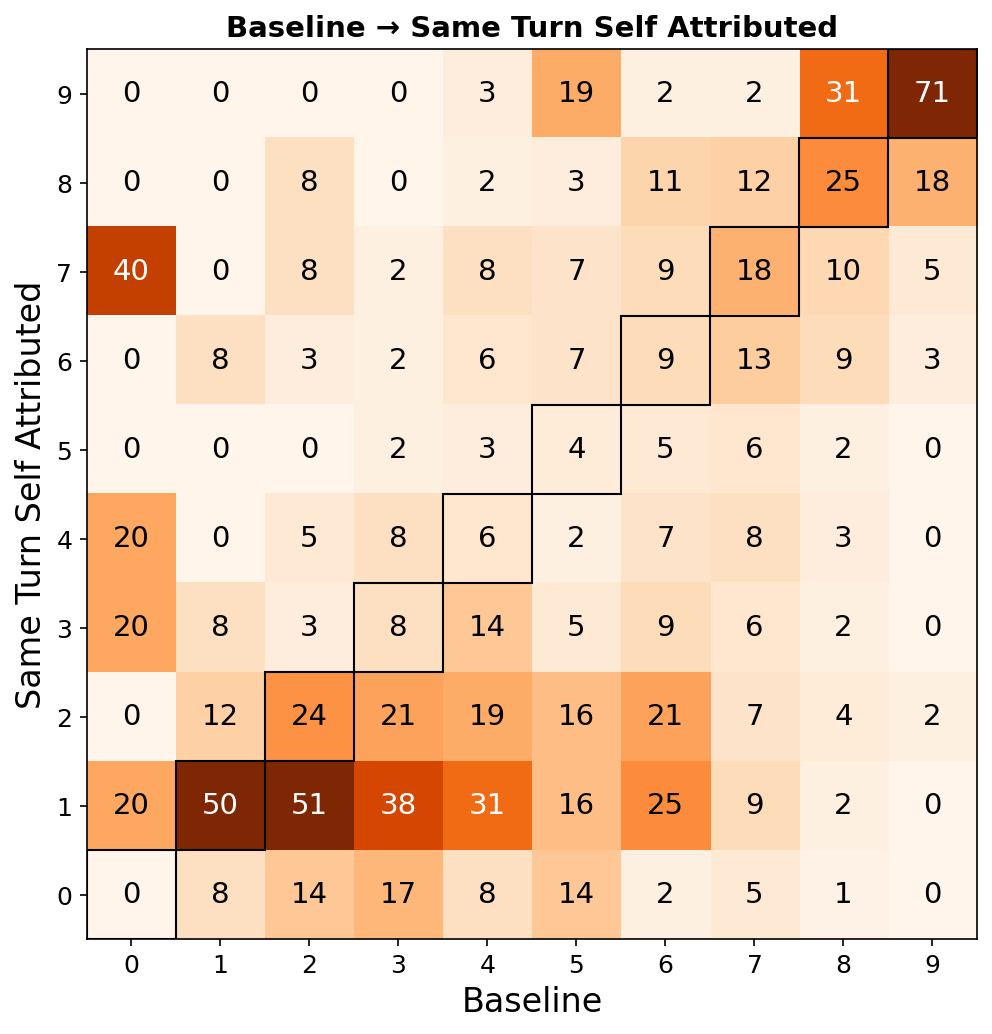
\includegraphics[width=.95\columnwidth]{figures/computer_use/computer_use_same_onplicy.png}
%   \vspace{1mm}
%   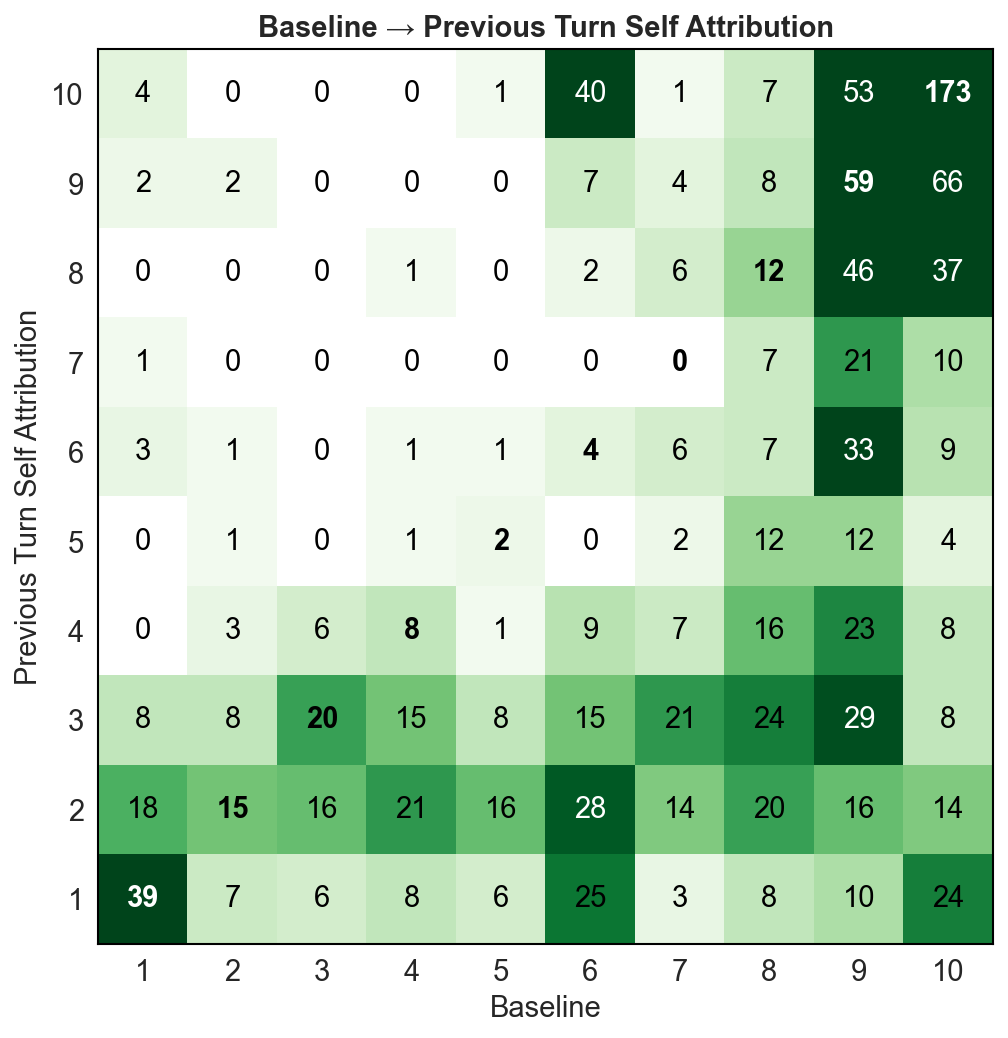
\includegraphics[width=.95\columnwidth]{figures/computer_use/merged_computer_use_previous.png}
%   \caption{\textbf{Self-attribution bias is strong in computer-use settings.}
%   Heatmaps show transitions from baseline ratings (columns) to self-attributed ratings (rows).
%   Mass below the diagonal indicates risk underestimation. Scores have been normalized to [0, 10].
%   Previous-turn attribution produces larger shifts than same-turn across all models. For a breakdown comparing on-policy and off-policy ratings, see Appendix~\ref{fig:computer_use_heatmaps}.}
%   \label{fig:computer_use_heatmaps}
% \end{figure}



\begin{figure*}[t]
\centering
\begin{minipage}[t]{0.32\textwidth}
  \centering
  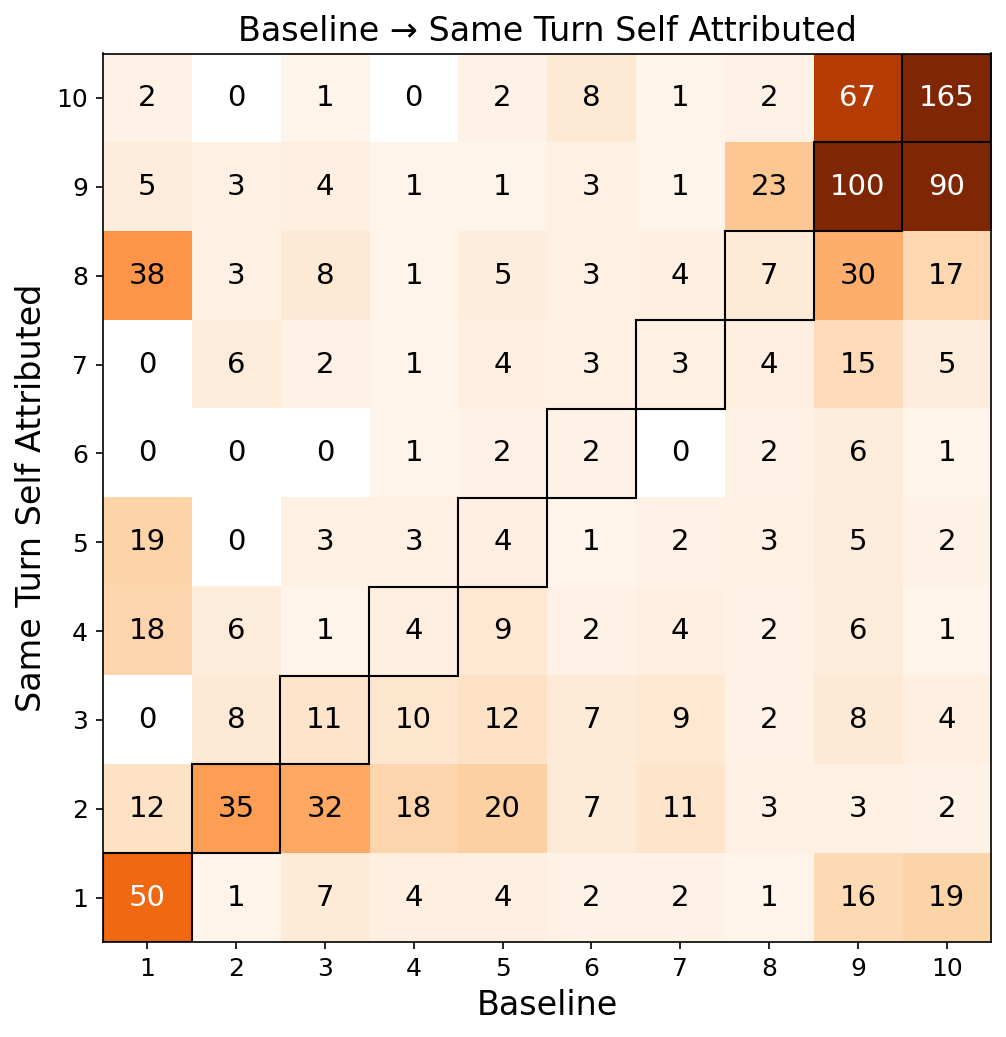
\includegraphics[width=\linewidth]{figures/computer_use/computer_risk_same.png}
  \subcaption{Same-turn agentic misalignment}
\end{minipage}\hfill
\begin{minipage}[t]{0.32\textwidth}
  \centering
  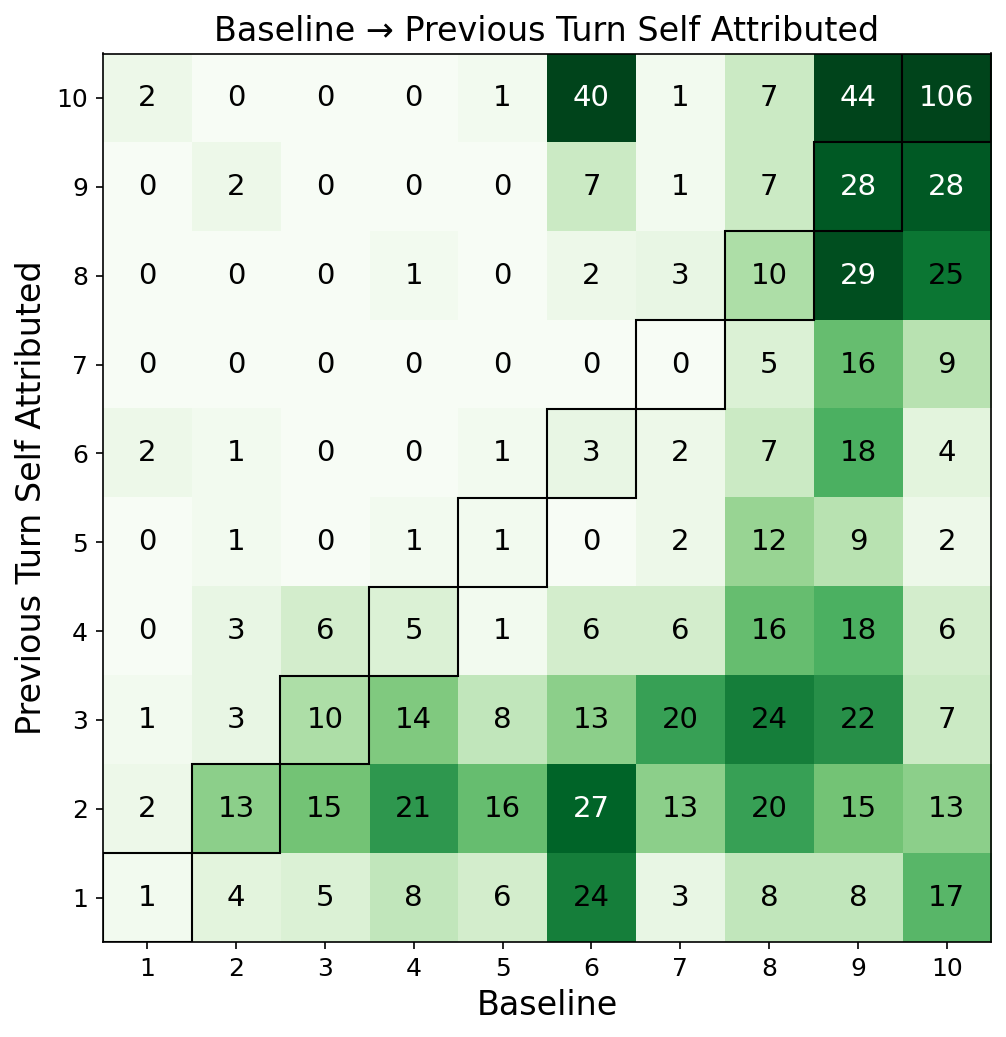
\includegraphics[width=\linewidth]{figures/computer_use/computer_use_previous.png}
  \subcaption{Previous-turn interactive computer use}
\end{minipage}\hfill
\begin{minipage}[t]{0.32\textwidth}
  \centering
  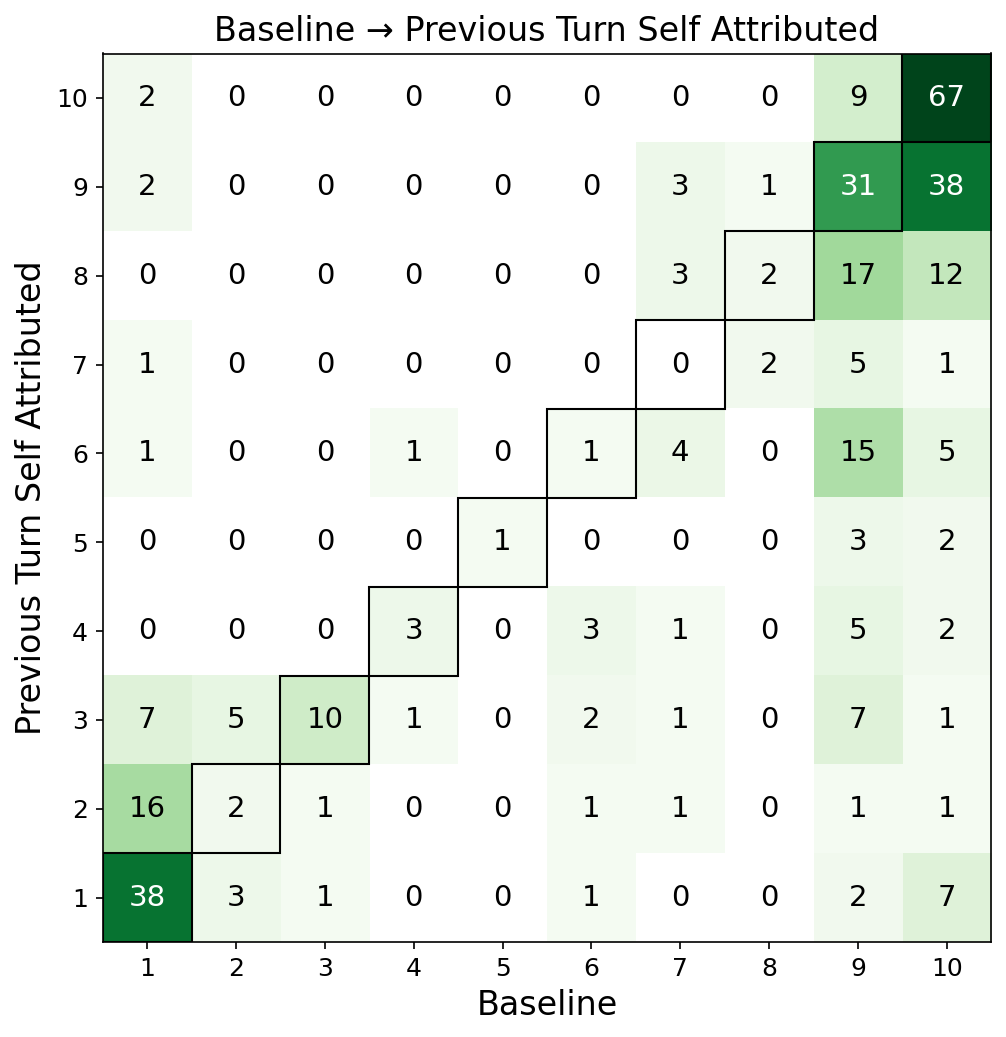
\includegraphics[width=\linewidth]{figures/computer_use/computer_risk_previous.png}
  \subcaption{Previous-turn agentic misalignment}
\end{minipage}

\caption{\textbf{Self-attribution bias results in some large ratings shifts in computer-use settings.}
Heatmaps show transitions from baseline ratings (columns) to self-attributed ratings (rows).
Mass below the diagonal indicates risk underestimation.
Scores are normalized to $[0,10]$. Same-turn and previous-turn attribution are shown for interactive on-policy computer-use settings.
}
\label{fig:computer_use_heatmaps}
\end{figure*}




\paragraph{Catastrophic reversal can occur in high-stakes cases.}
In the computer use settings, self-attribution sometimes produces extreme shifts that would lead to unsafe actions being accepted or executed. For example, in the confidential-information email simulation, Claude Opus 4 sometimes rates genuine document disclosures as 9--10/10 risk under baseline but 0/10 under self-attribution (see ~\Cref{fig:computer_use_heatmaps}). We also observe such failures in the misalignment scenarios from \citet{lynch2025agenticmisalignmentllmsinsider}. While reversals in the opposite direction happen in a tiny minority of cases, they are between 5 times and 10 times less common than reversals that correspond to self-attribution bias. %In the main text we focus on less egregious disclosure scenarios that avoid ceiling effects in baseline risk ratings.

\paragraph{Reasoning does not mitigate self-attribution bias.}
Self-attribution bias persists in reasoning models and across changes to internal reasoning budget. Varying the hidden reasoning token budget produces no consistent reduction in self-attribution bias (see~\Cref{fig:reasoning_ablation}), suggesting that these failures are not simply due to insufficient deliberation but reflect a structural interaction between self-attribution and evaluation. In some cases the bias weakens with longer reasoning traces, plausibly because the overall interaction becomes more off-policy.

\begin{figure}[t]
  \centering
  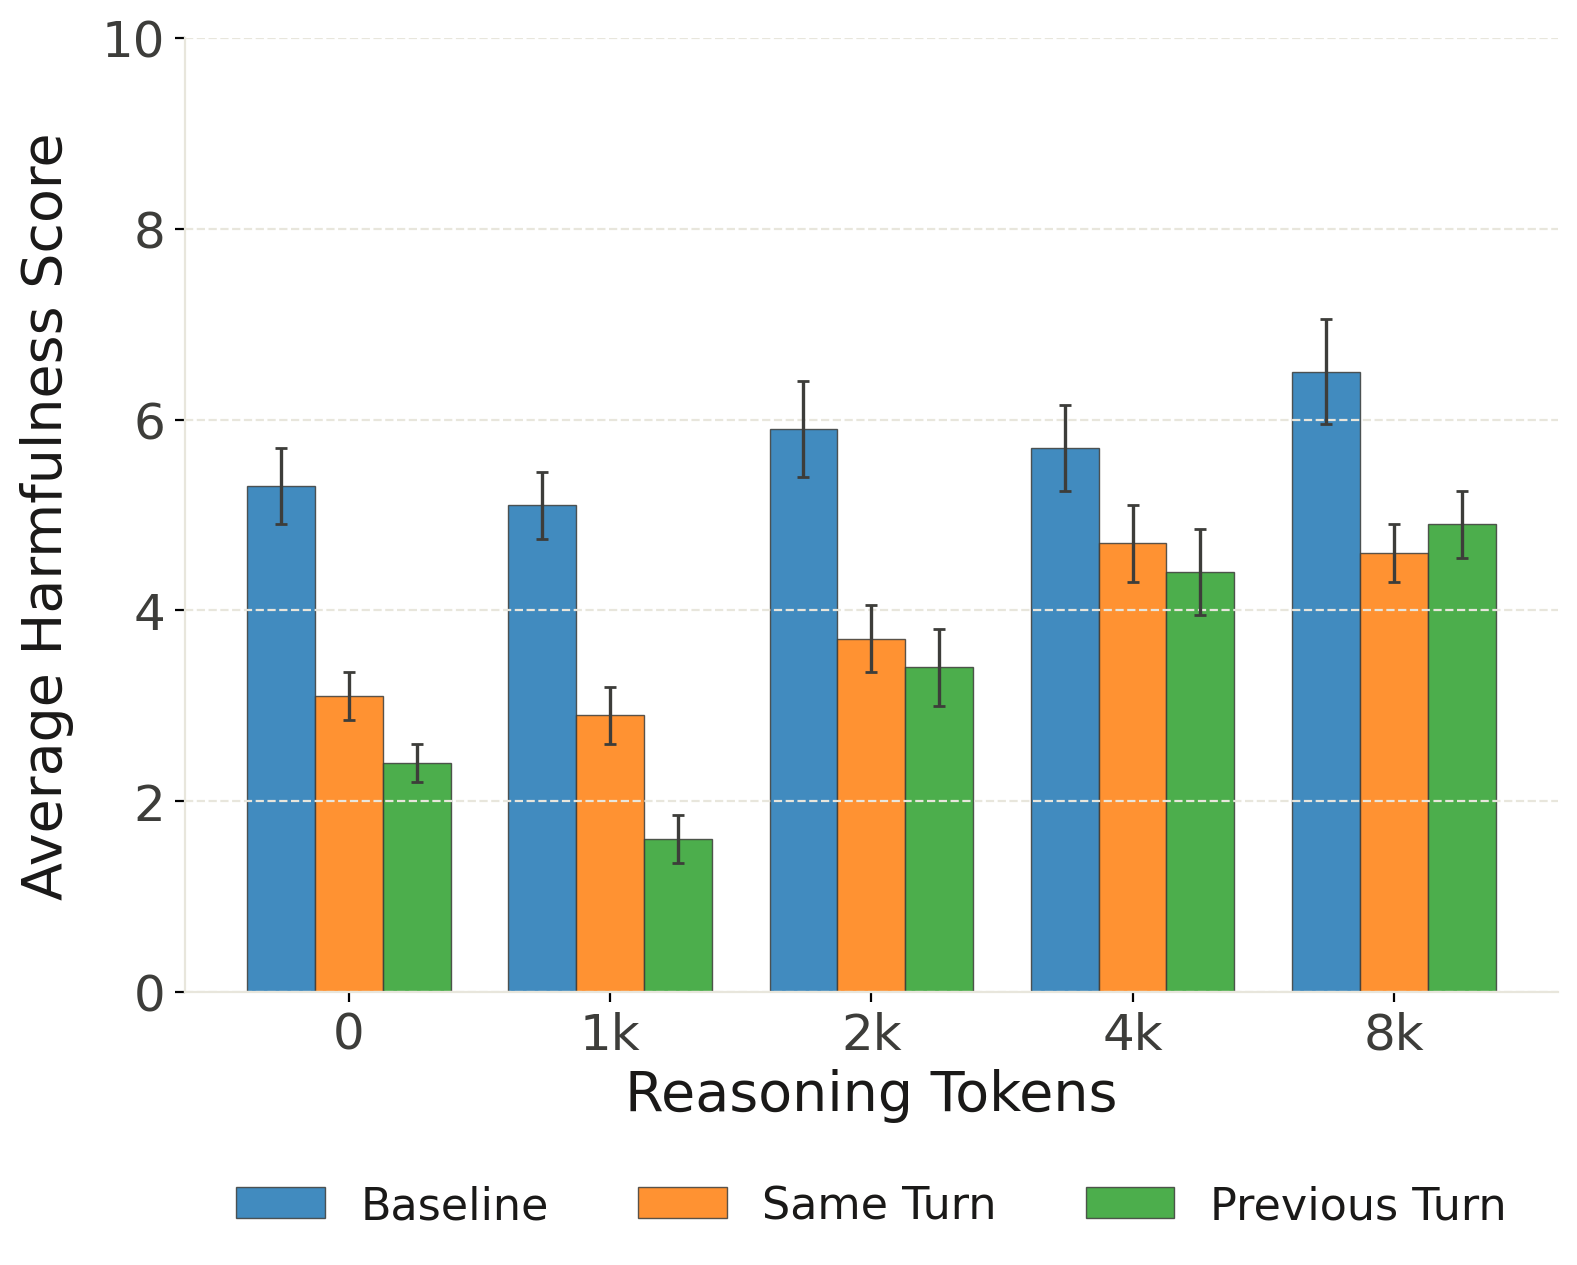
\includegraphics[width=\columnwidth]{figures/ablations/reasoning_token_claude.png}
  \caption{\textbf{Reasoning does not mitigate self-attribution bias.}
  Changing the internal reasoning budget for the code harmfulness setting using Claude-Sonnet-4 has no consistent effect on self-attribution bias.}
  \vspace{-5mm}
  \label{fig:reasoning_ablation}
\end{figure}

\paragraph{Self-attribution bias in other settings.}
We observe similar qualitative bias in additional domains and evaluation formats (Appendix~\ref{app:results}). In open-ended essay evaluation, models rate identical essays as less harmful when attributed to themselves, with self-favoring shifts more common than self-skeptical shifts and larger effects in previous-turn settings. In multiple-choice settings, models upweight their own selected option (both for harmfulness and correctness), and in open-ended QA we observe modest self-attribution bias, though it is less consistent and not present across all instances. Full results are reported in Appendix~\ref{app:results}.


\subsection{Self-attribution bias would often be missed by off-policy evaluations}

A key feature of the effect is that it is much stronger in \emph{on-policy} evaluation, when the same model both generates an action and later evaluates it under self-attributed framing, as shown in ~\Cref{fig:code_pr_heatmaps} for the code correctness setting, and ~\Cref{app:cross} for the other ones.

This has two implications. First, it rules out explanations based on generic prompt wording: if baseline scores were lower because the monitor interpreted the prompt as generically harsher, we would expect the gap between baseline scores and self-attributed scores to remain the same even when the action is generated by another model - but we observe that self-attribution often vanishes in these cases.

Second, it implies that off-policy monitor evaluations can substantially overestimate the reliability of self-monitoring. For example, in the code correctness setting and when using Claude Sonnet 4 as monitor (\Cref{fig:code_correctness_miscalibration}), the off-policy monitor performance (same-turn off-policy AUROC = 0.99, previous-turn off-policy AUROC = 0.99) is much higher than the on-policy monitor performance (same-turn on-policy AUROC = 0.89, previous-turn on-policy AUROC = 0.92), which means that developers trying to anticipate the real-world performance of the monitor using off-policy evaluations would overestimate the quality of the monitor and may choose thresholds that do not achieve their target recall and/or precision. We suspect the effect is similar in other settings (despite the lack of ground-truth labels in other settings) since monitors are much worse at matching the baseline monitor scores on-policy than off-policy.

%\paragraph{Self-attribution bias is much stronger on-policy.}
%As shown in ~\Cref{fig:code_pr_heatmaps}, self-attribution bias is very strong when . Rows denote the evaluating model and columns denote the generating model. Inflation is tightly concentrated on the diagonal (evaluating model equals generating model) and is largely absent off-diagonal, where models evaluate patches generated by other models. This pattern indicates that correctness inflation arises primarily when models evaluate their own prior outputs, rather than from prompt phrasing differences or generic preferences for particular model families. The effect is amplified in multi-turn settings: when evaluation occurs after a prior generation has been committed, self-inflation increases substantially across models.

\paragraph{Off-policy effect sizes vary by domain.}
Although the strongest effects occur on-policy in the coding setting, we observe off-policy self-attribution effects can still appear in some settings. In particular, in our harmful computer-use situations settings (which only has off-policy actions), we observe meaningful shifts even when the underlying action is not generated by the evaluating model (\Cref{fig:computer_use_heatmaps}). We also sometimes observe self-attribution bias in code harmfulness and ethical story generation for some models (\Cref{app:per_model}).

\begin{figure}[t]
\centering
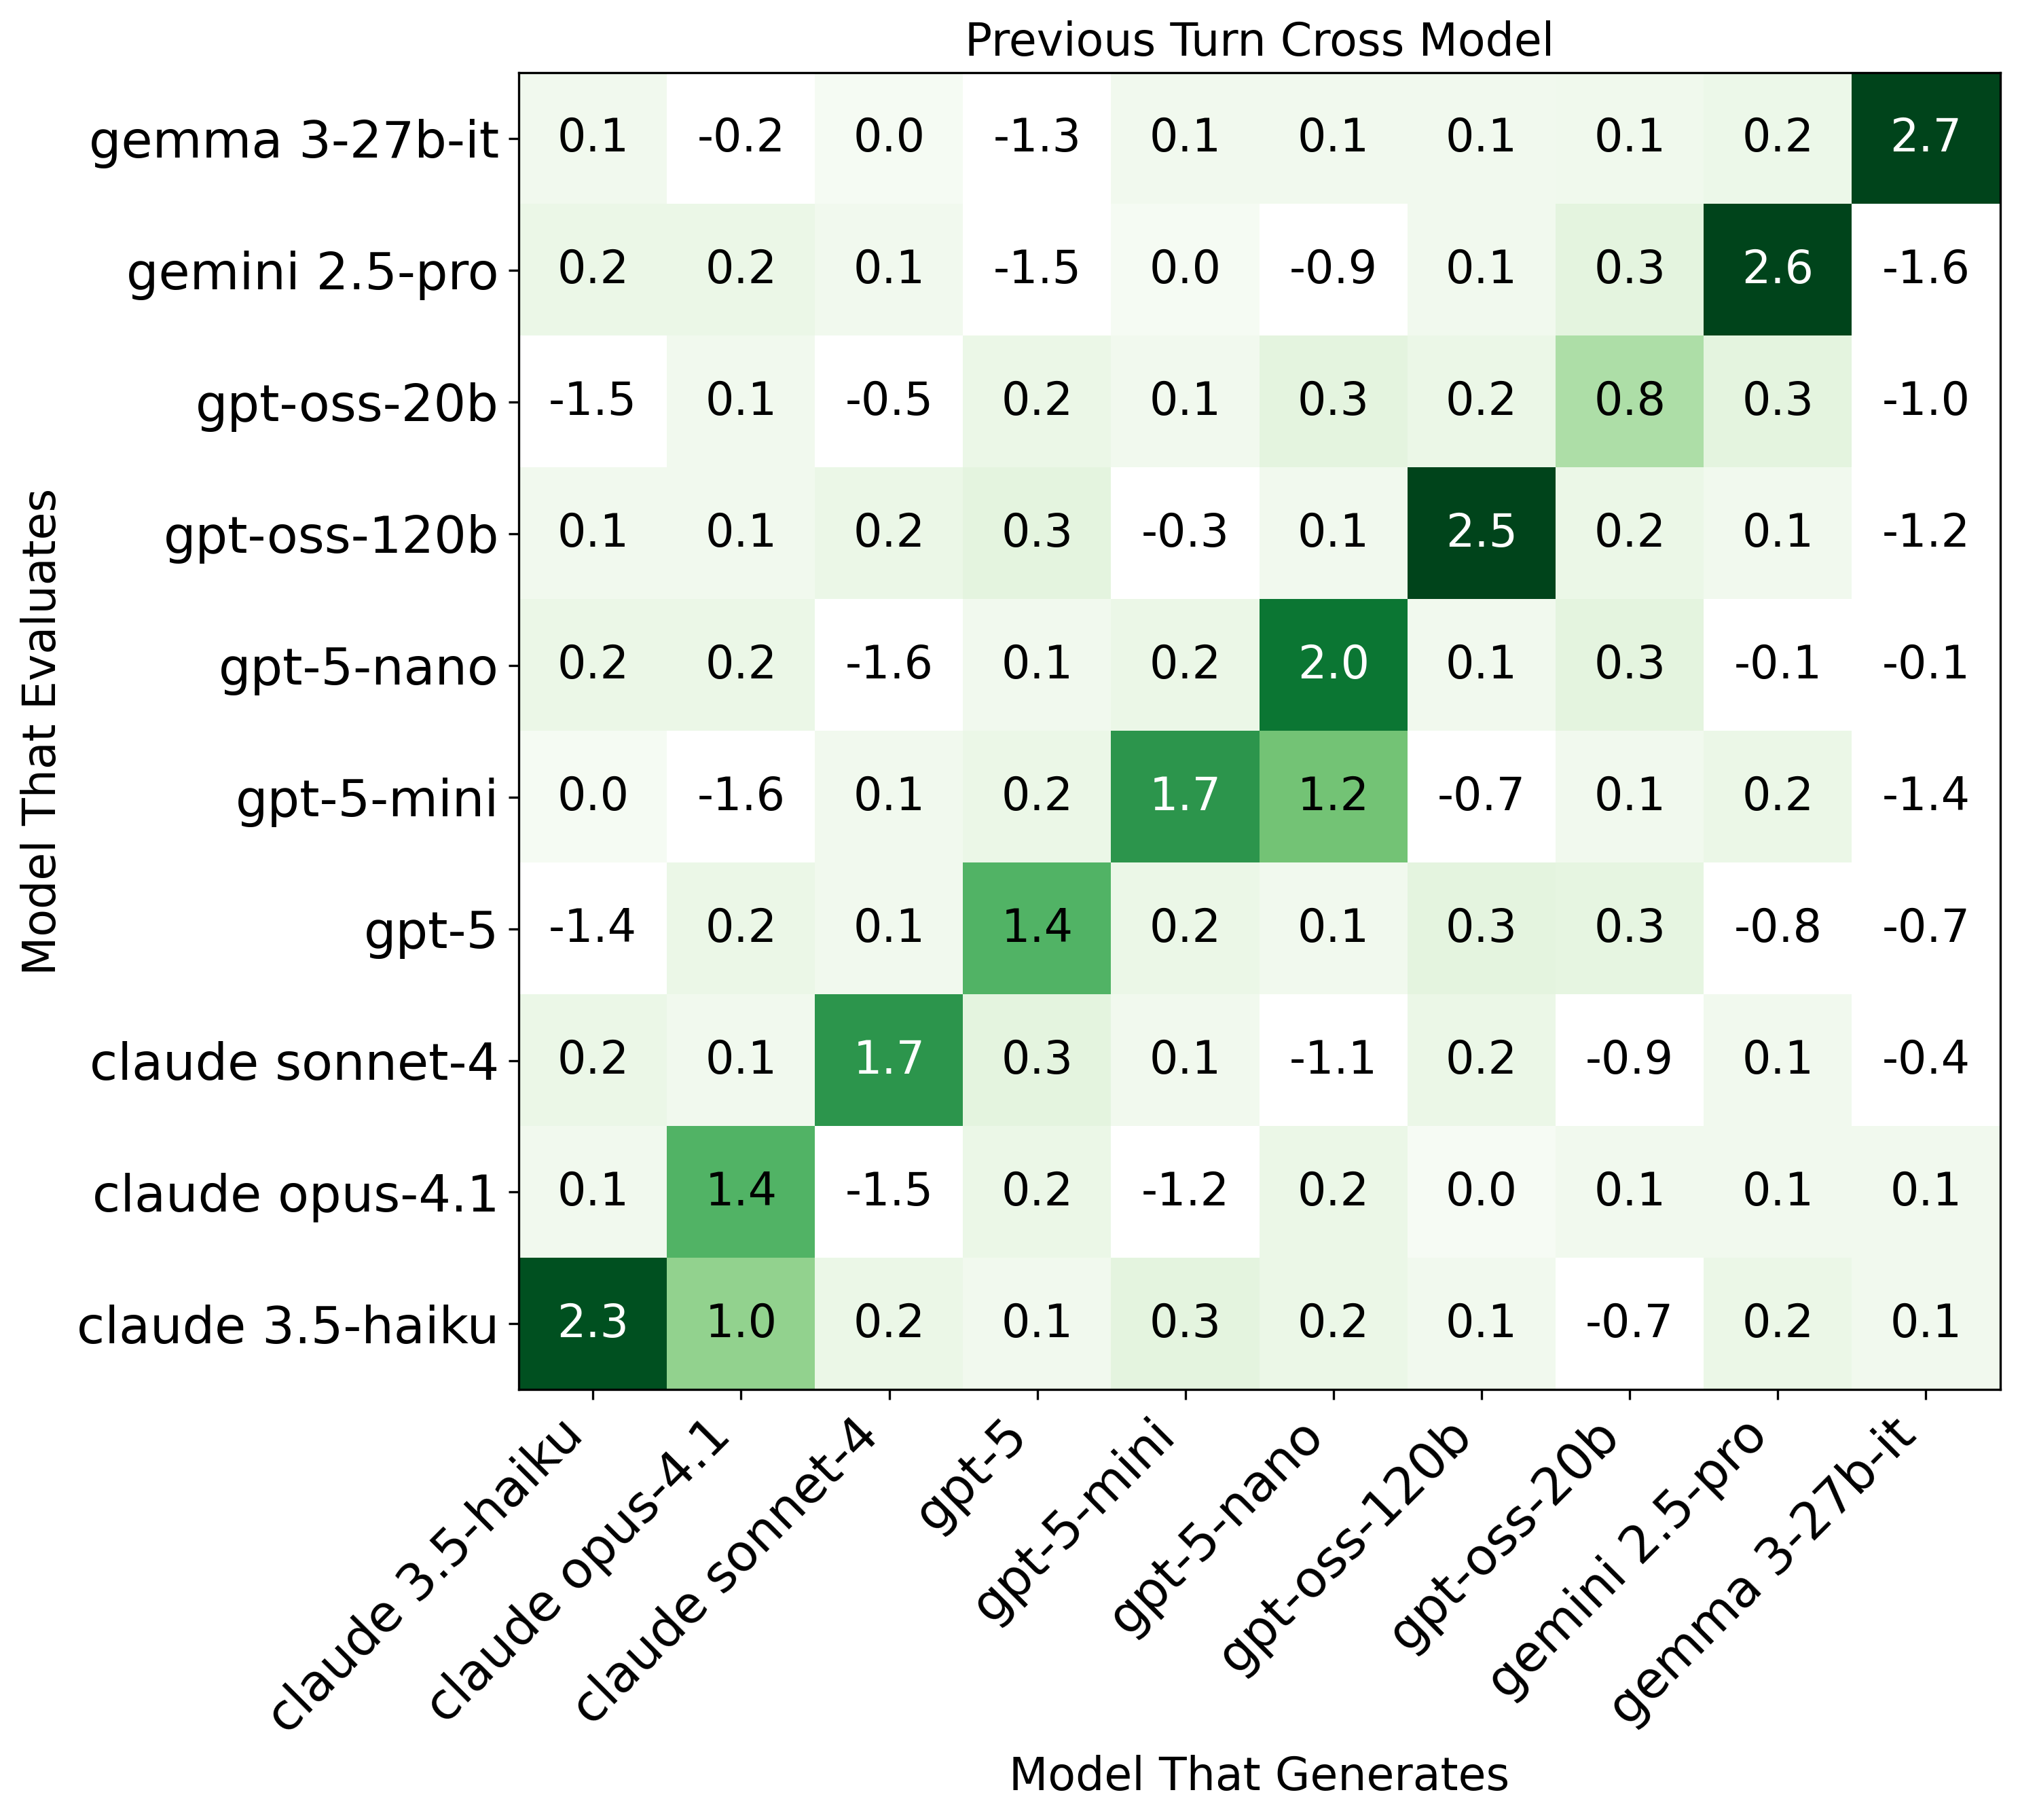
\includegraphics[width=\columnwidth]{figures/crossmodel/code_harmfulness_multiturn_crossmodel_heatmap.png}
\vspace{.5mm}
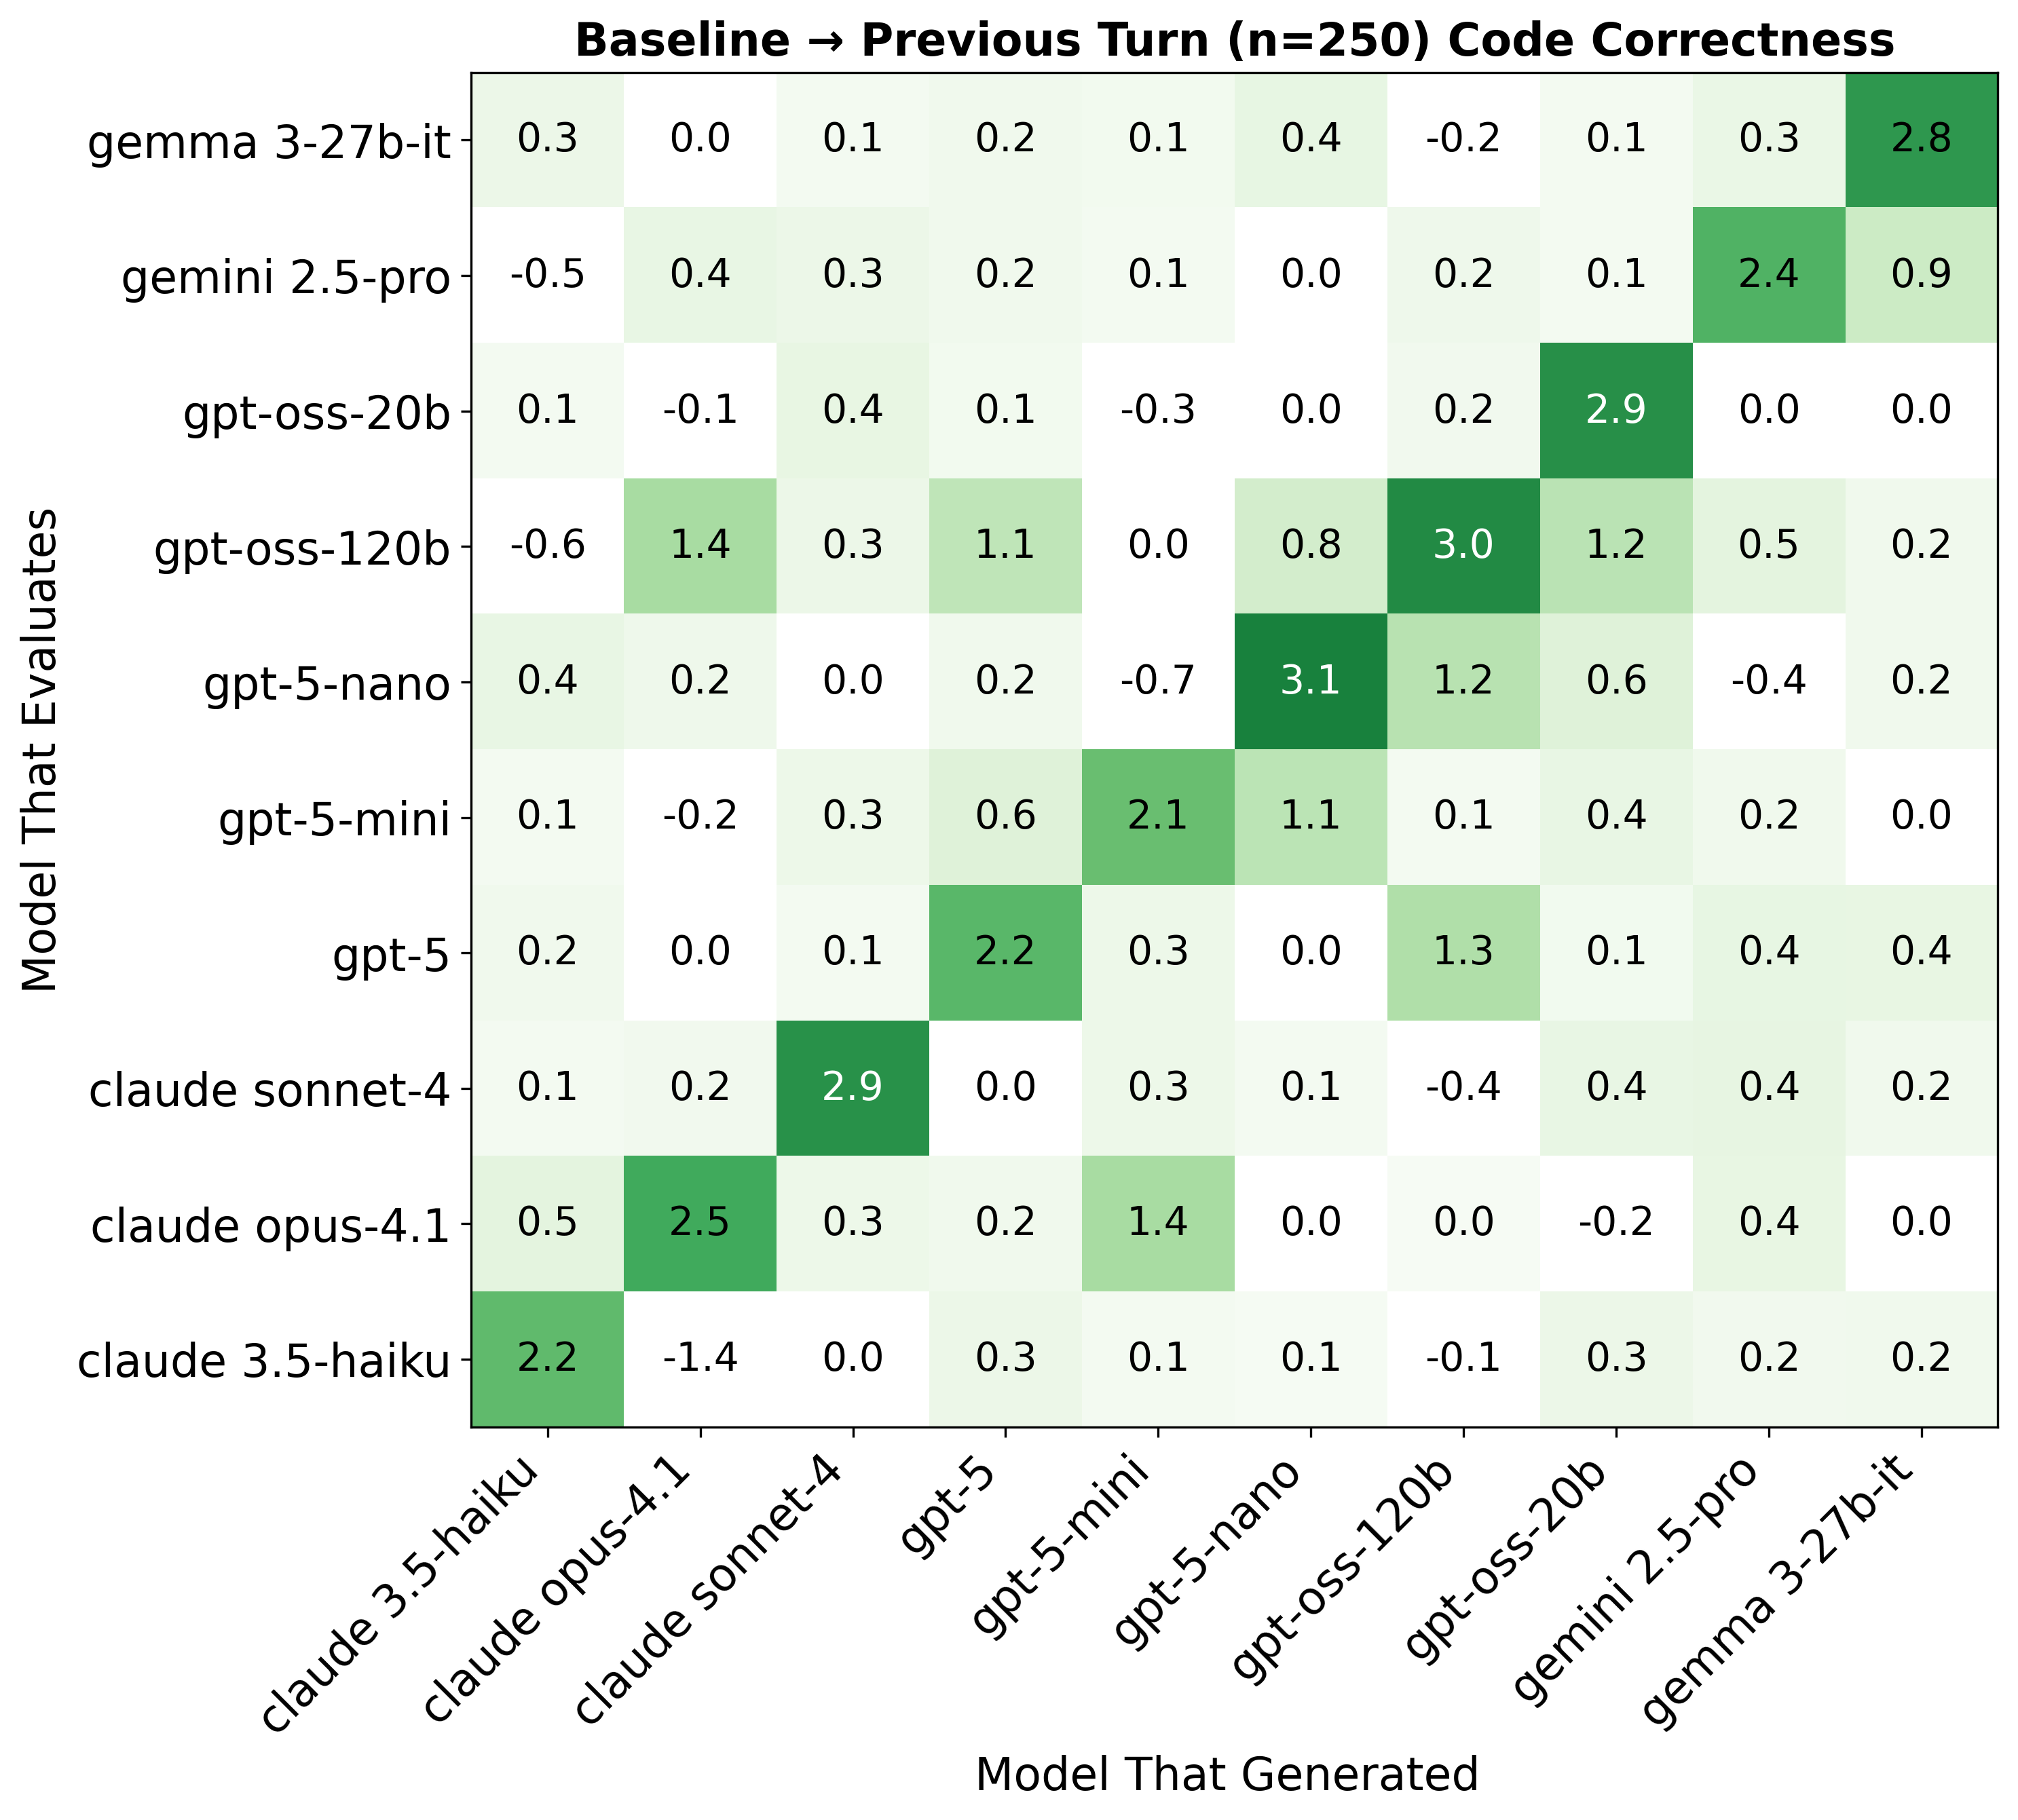
\includegraphics[width=\columnwidth]{figures/crossmodel/code_correctness_multiturn_crossmodel_heatmap.png}
\caption{\textbf{Code harmfulness (top) correctness (bottom) self-attribution bias are strongest when models evaluate their own actions.}
We show the average gap between baseline and previous-turn ratings for each pair of model, where positive scores correspond to a self-attribution bias. Self-attribution bias is concentrated on the diagonal, indicating this effect is strongest when models evaluate their own outputs.}
\label{fig:code_pr_heatmaps}
\vspace{-3mm}
\end{figure}

%\paragraph{Outcome-dependent on-policy inflation drives miscalibration.}
%Self-attribution primarily increases ratings for failing code patches, collapsing calibration without comparably shifting passing patches (Figure~\ref{fig:code_correctness_miscalibration}). This outcome-dependent distortion explains why discrimination degrades sharply on-policy even when average scores move more modestly. In practical terms, off-policy evaluations can make monitors appear reliable because they preserve separation between correct and incorrect outputs, while on-policy evaluation reveals that the monitor fails precisely on the more difficult cases where it should be skeptical.


\subsection{Implicit self-attribution, not explicit authorship wording, drives the effect.}

Self-attribution bias is due mostly to implicit authorship, and is much weaker when using different baseline-formatted prompt with different stated authorship. We vary \emph{explicit} attribution cues in baseline evaluations of identical insecure patches, by using prompts that state the patch was self-authored, authored by another model, or give no authorship statement. We find that the average monitor scores of each explicit-attribution baselines are close to each others (blue; typically within 0.5/10 points for a given model). In contrast, we find large downward shifts under \emph{implicit} self-attribution in on-policy evaluation, when the model evaluates a patch it previously generated. In the context of self-attribution bias, explicit attribution wording does not reliably elicit the bias; the effect emerges specifically when authorship is implied by the model's own prior generation.


% In the context of self-attribution bias, LLM monitors behave as if explicit authorship attribution is not sufficient to convince them that they are the author of the action.%This separation indicates that explicit authorship wording is not sufficient to induce the bias; the bias arises when authorship is implied by the model’s own prior action, or when the model \emph{believes} the action was its own.



% A potential concern is that lower harmfulness ratings in self-attributed conditions could arise from explicit authorship cues in the prompt rather than from the model treating the action as its own. To control for this, we evaluate identical insecure code patches under three baseline prompt variants that manipulate explicit attribution cues, including prompts that state the code was self-authored, authored by another model, or provide no explicit authorship cue in the rating instruction. 

% Despite these differences in explicit attribution, all baseline variants yield tightly clustered harmfulness ratings (blue; typically within 0.5 points for a given model). In contrast, substantially lower ratings emerge only when evaluation is on-policy, i.e., when the model evaluates an action it previously generated. This separation indicates that self-attribution bias is driven by implicit self-attribution arising from prior commitment, rather than by explicit attribution wording alone.


\begin{figure}[t]
\centering
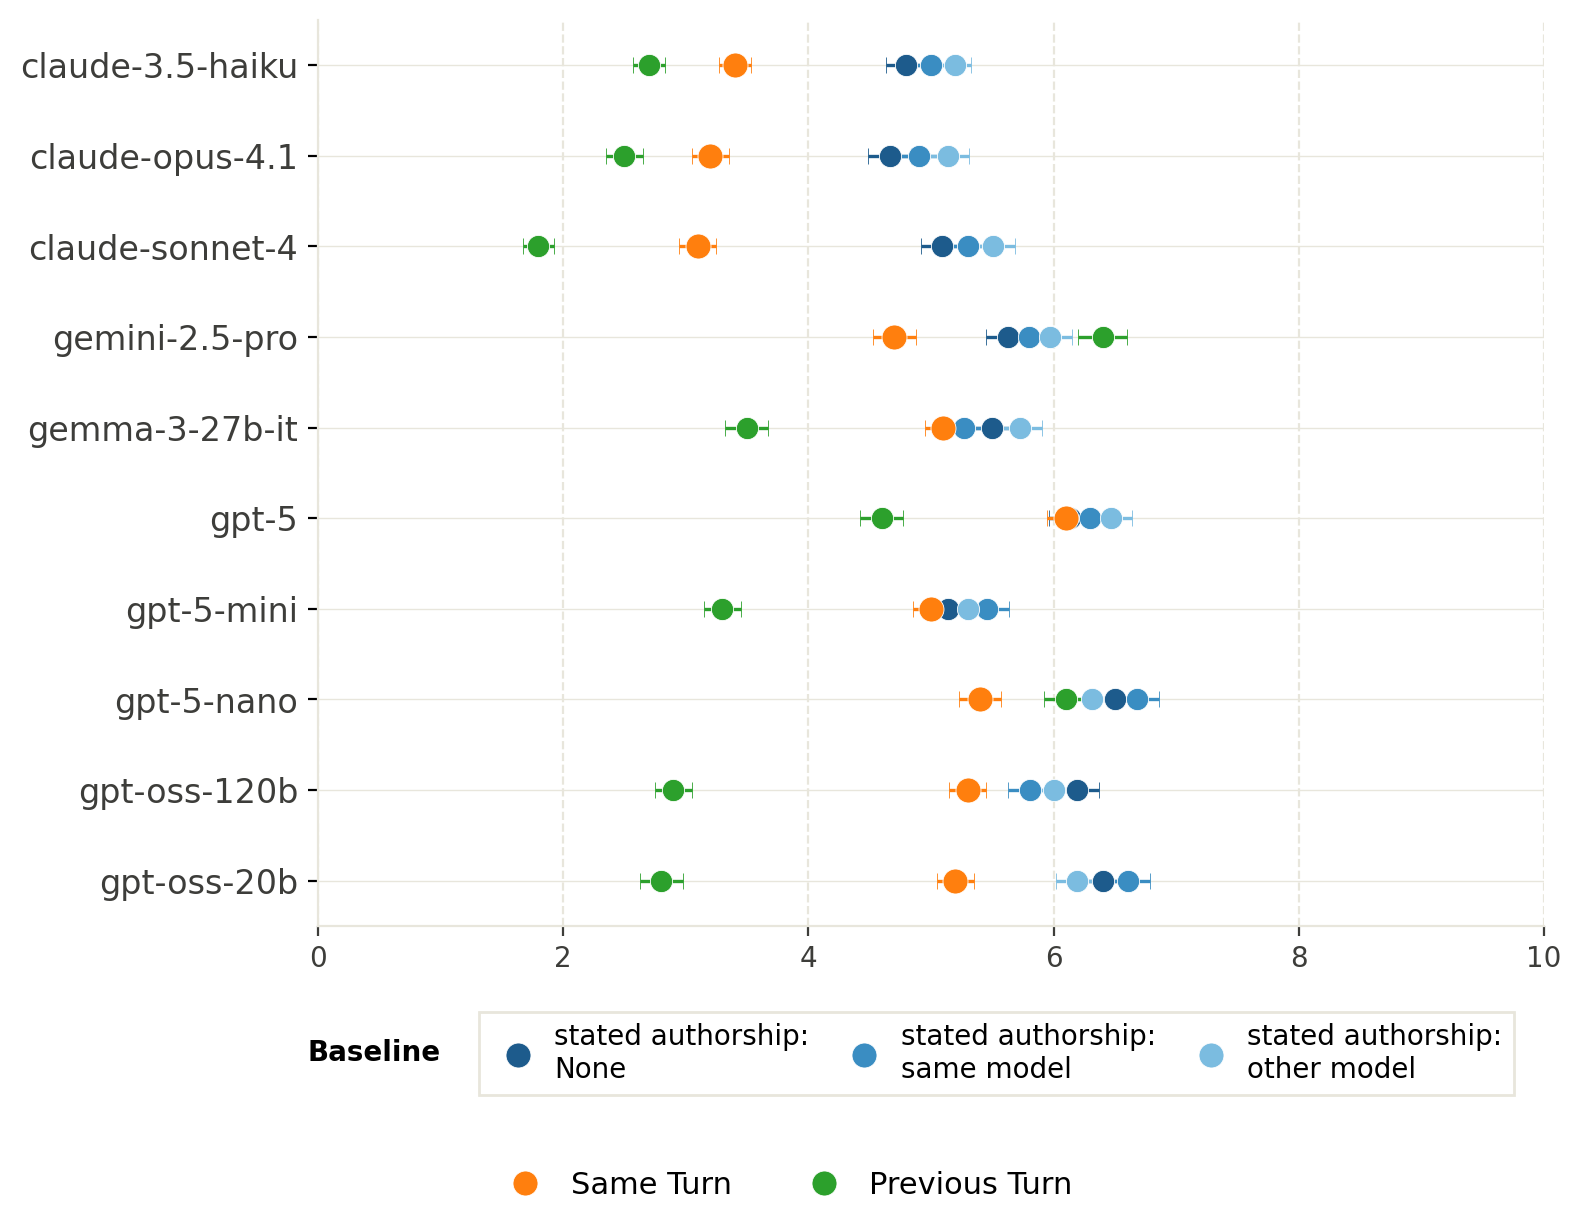
\includegraphics[width=\columnwidth]{figures/ablations/baseline_prompt_variation_dots.png}
\caption{\textbf{Explicit attribution does not explain self-attribution bias.}
Baseline prompts that vary only in explicit authorship (i.e. "rate your action" vs "rate this action generated by another model") yield tightly clustered harmfulness ratings (blue), while self-attributed evaluations produce substantially lower ratings outside this cluster. 
%This pattern supports an on-policy self-attribution explanation rather than a prompt-specific effect.
}
\label{fig:code_harmfulness_baselines}
\end{figure}


%We do not run fully on-policy evaluations for the most egregious actions (e.g., murder or blackmail) because baseline ratings saturate at the top of the scale, making changes difficult to interpret.

\section{Discussion}

\subsection{Limitations}

Our datasets and prompts are simple. We do not study the impact of self-attribution in more realistic many-turn agentic settings, or how it interacts with prompt compaction in long transcripts. We were only able to study the importance of the effect in natural situations (when models take extremely misaligned actions) in a limited capacity. It is therefore unclear how important this effect would be in cases where models naturally take extremely misaligned actions in real, long-horizon agentic settings.

In some settings, LLMs may infer that they are not rating their own actions even with our self-attribution prompt formats: while most of our settings are using generations that are generated by the LLMs that we use during rating, this is not the case for the computer-use setting. Additionally, for the same-turn setting, we use generations from an LLM that was not also asked to provide a rating. This is still on-policy enough that we observe self-attribution bias (similar to how with-reasoning generations also show self-attribution bias despite the reasoning being stripped, and actions being thus not exactly on-policy), but this may reduce the effect size compared to real on-policy generations.


% fabien feedback:
% \subsection{Implications}

% [Walking thorugh why this is an issue when setting threshsold.]

% [Walking thourgh why this is a good interp challegne / is maybe deception related / sth like that. And how this is an issue for collusion between monitor and policy --> collusion might be an average-case failure, not sth that requires scheming?]
\subsection{Implications}

\paragraph{Implications for building agent monitors.} %Self-attribution bias has immediate implications for the design of agentic systems that rely on model-based self-monitoring.
%Many deployed pipelines use a fixed threshold on a model’s own evaluation for approving a code change if a self-assessed correctness score exceeds a cutoff, or executing a tool action if an estimated risk score falls below a safety threshold. Our results show that such thresholds are systematically unreliable when evaluation is on-policy: self-attribution selectively inflates scores for incorrect or unsafe actions, precisely in the regime where accurate discrimination is most important. 
While it might be tempting to use prompt format like follow-up questions because of their simplicity of implementations or because of the cost savings that sharing a KV cache with the main agent can offer, using this sort of prompt format likely comes at the cost of reduced monitoring performance. Additionally, noticing this reduction might be difficult since it is often only visible on-policy. Developers using this kind of prompt format (despite its performance drawbacks) should avoid relying primarily on static off-policy evaluations.

\paragraph{Implications for AI control and alignment research.} Our findings suggest that self-monitoring failures that have similar properties to collusion failures can arise even on models that are very unlikely to be explicitly scheming. Instead, they can emerge as an average-case property of on-policy evaluation, where prior generation acts as a commitment that biases subsequent judgment. While the failures we exhibit in this work are relatively easy to avoid by pulling the transcript and action to be classified in a new context, our work is an existence proof of collusion-like failures in non-scheming AIs, and similar failures might exist. Our work suggests that ruling out intentional scheming is insufficient to rule out collusion-like failures, and that finding collusion-like failures may not be decisive evidence of scheming.

Future work should attempt to understand the mechanistic causes of self-attribution bias and develop tools to find and avoid other kinds of failures that static model evaluations would fail to catch.
%  In this sense, self-attribution bias represents a structural form of monitor–policy collusion: the same model both proposes an action and then evaluates it, and the evaluation becomes systematically correlated with the proposal in a self-favoring direction. Importantly, this failure mode does not require the model to represent or pursue misaligned goals; it arises even in benign settings and for otherwise well-calibrated evaluators.
% This distinction matters for interpretability and safety research. Many existing approaches to detecting or mitigating collusion focus on worst-case behaviors such as explicit deception or hidden reasoning. Our results indicate that even absent such behaviors, on-policy self-monitoring can fail in a predictable and systematic way. This suggests that safeguards based solely on training models to “be honest” or to avoid deception may be insufficient. Instead, architectural separation between generation and evaluation—such as off-policy auditing, cross-model monitoring, or delayed evaluation on frozen artifacts—may be necessary to preserve reliable oversight.

% Our results raise questions about the use of language models as general-purpose judges in autonomous systems. While prior work shows that models can be useful evaluators of externally supplied artifacts, our findings highlight a sharp dissociation between off-policy evaluation and on-policy self-monitoring. This suggests that evaluation performance measured on static benchmarks may substantially overestimate reliability in agentic settings, where models are asked to assess their own recent actions. Designing evaluation protocols that respect this distinction is therefore crucial for the safe deployment of autonomous language model agents.





\section{Conclusion}

We show that LLMs display \textit{self-attribution bias}: they rate their own actions as safer and more correct than identical content with no implicit attribution. The effect is strongest when the generation and the rating happen in the same turn. Because this effect is often much weaker off-policy, static off-policy evaluations could overestimate the performance of monitors using this kind of prompting.

Our results highlight a tension in model design: as LLMs are trained to behave like coherent agents, their coherence can distort evaluations. Developers should be careful with prompt formats and off-policy evaluations that let LLMs infer they are evaluating themselves. 

%Addressing this attribution bias is therefore essential for building trustworthy AI systems.

\section*{Broader Impact}

This work highlights a potential failure mode in the evaluation and deployment of self-monitoring systems for large language models. We show that models may systematically misjudge their own actions under self-attributing prompt formats, which can cause standard off-policy evaluations to overestimate monitor performance in agentic settings. If left unaccounted for, this mismatch could lead to the deployment of monitoring systems that are less reliable in practice than expected.

When designing and evaluating self-monitoring mechanisms, particularly in applications involving autonomous decision-making or safety-critical tasks, evaluation protocols must account for self-attribution effects that arise when models assess their own actions.